\documentclass[
  man,
  floatsintext,
  longtable,
  nolmodern,
  notxfonts,
  notimes,
  colorlinks=true,linkcolor=blue,citecolor=blue,urlcolor=blue]{apa7}

\usepackage{amsmath}
\usepackage{amssymb}
\usepackage{setspace}


\usepackage[bidi=default]{babel}
\babelprovide[main,import]{english}


% get rid of language-specific shorthands (see #6817):
\let\LanguageShortHands\languageshorthands
\def\languageshorthands#1{}

\RequirePackage{longtable}
\RequirePackage{threeparttablex}

\usepackage{framed}


\makeatletter
\renewcommand{\paragraph}{\@startsection{paragraph}{4}{\parindent}%
	{0\baselineskip \@plus 0.2ex \@minus 0.2ex}%
	{-.5em}%
	{\normalfont\normalsize\bfseries\typesectitle}}

\renewcommand{\subparagraph}[1]{\@startsection{subparagraph}{5}{0.5em}%
	{0\baselineskip \@plus 0.2ex \@minus 0.2ex}%
	{-\z@\relax}%
	{\normalfont\normalsize\bfseries\itshape\hspace{\parindent}{#1}\textit{\addperi}}{\relax}}
\makeatother




\usepackage{longtable, booktabs, multirow, multicol, colortbl, hhline, caption, array, float, xpatch}
\usepackage{subcaption}


\renewcommand\thesubfigure{\Alph{subfigure}}
\setcounter{topnumber}{2}
\setcounter{bottomnumber}{2}
\setcounter{totalnumber}{4}
\renewcommand{\topfraction}{0.85}
\renewcommand{\bottomfraction}{0.85}
\renewcommand{\textfraction}{0.15}
\renewcommand{\floatpagefraction}{0.7}

\usepackage{tcolorbox}
\tcbuselibrary{listings,theorems, breakable, skins}
\usepackage{fontawesome5}

\definecolor{quarto-callout-color}{HTML}{909090}
\definecolor{quarto-callout-note-color}{HTML}{0758E5}
\definecolor{quarto-callout-important-color}{HTML}{CC1914}
\definecolor{quarto-callout-warning-color}{HTML}{EB9113}
\definecolor{quarto-callout-tip-color}{HTML}{00A047}
\definecolor{quarto-callout-caution-color}{HTML}{FC5300}
\definecolor{quarto-callout-color-frame}{HTML}{ACACAC}
\definecolor{quarto-callout-note-color-frame}{HTML}{4582EC}
\definecolor{quarto-callout-important-color-frame}{HTML}{D9534F}
\definecolor{quarto-callout-warning-color-frame}{HTML}{F0AD4E}
\definecolor{quarto-callout-tip-color-frame}{HTML}{02B875}
\definecolor{quarto-callout-caution-color-frame}{HTML}{FD7E14}

%\newlength\Oldarrayrulewidth
%\newlength\Oldtabcolsep


\usepackage{hyperref}
\usepackage[protrusion=true]{microtype}



\providecommand{\tightlist}{%
  \setlength{\itemsep}{0pt}\setlength{\parskip}{0pt}}
\usepackage{longtable,booktabs,array}
\newcounter{none} % for unnumbered tables
\usepackage{calc} % for calculating minipage widths
% Correct order of tables after \paragraph or \subparagraph
\usepackage{etoolbox}
\makeatletter
\patchcmd\longtable{\par}{\if@noskipsec\mbox{}\fi\par}{}{}
\makeatother
% Allow footnotes in longtable head/foot
\IfFileExists{footnotehyper.sty}{\usepackage{footnotehyper}}{\usepackage{footnote}}
\makesavenoteenv{longtable}

\usepackage{graphicx}
\makeatletter
\newsavebox\pandoc@box
\newcommand*\pandocbounded[1]{% scales image to fit in text height/width
  \sbox\pandoc@box{#1}%
  \Gscale@div\@tempa{\textheight}{\dimexpr\ht\pandoc@box+\dp\pandoc@box\relax}%
  \Gscale@div\@tempb{\linewidth}{\wd\pandoc@box}%
  \ifdim\@tempb\p@<\@tempa\p@\let\@tempa\@tempb\fi% select the smaller of both
  \ifdim\@tempa\p@<\p@\scalebox{\@tempa}{\usebox\pandoc@box}%
  \else\usebox{\pandoc@box}%
  \fi%
}
% Set default figure placement to htbp
\def\fps@figure{htbp}
\makeatother


% definitions for citeproc citations
\NewDocumentCommand\citeproctext{}{}
\NewDocumentCommand\citeproc{mm}{%
  \begingroup\def\citeproctext{#2}\cite{#1}\endgroup}
\makeatletter
 % allow citations to break across lines
 \let\@cite@ofmt\@firstofone
 % avoid brackets around text for \cite:
 \def\@biblabel#1{}
 \def\@cite#1#2{{#1\if@tempswa , #2\fi}}
\makeatother
\newlength{\cslhangindent}
\setlength{\cslhangindent}{1.5em}
\newlength{\csllabelwidth}
\setlength{\csllabelwidth}{3em}
\newenvironment{CSLReferences}[2] % #1 hanging-indent, #2 entry-spacing
 {\begin{list}{}{%
  \setlength{\itemindent}{0pt}
  \setlength{\leftmargin}{0pt}
  \setlength{\parsep}{0pt}
  % turn on hanging indent if param 1 is 1
  \ifodd #1
   \setlength{\leftmargin}{\cslhangindent}
   \setlength{\itemindent}{-1\cslhangindent}
  \fi
  % set entry spacing
  \setlength{\itemsep}{#2\baselineskip}}}
 {\end{list}}
\usepackage{calc}
\newcommand{\CSLBlock}[1]{\hfill\break\parbox[t]{\linewidth}{\strut\ignorespaces#1\strut}}
\newcommand{\CSLLeftMargin}[1]{\parbox[t]{\csllabelwidth}{\strut#1\strut}}
\newcommand{\CSLRightInline}[1]{\parbox[t]{\linewidth - \csllabelwidth}{\strut#1\strut}}
\newcommand{\CSLIndent}[1]{\hspace{\cslhangindent}#1}


\usepackage[nolongtablepatch]{lineno}

\linenumbers



\usepackage{newtx}

\defaultfontfeatures{Scale=MatchLowercase}
\defaultfontfeatures[\rmfamily]{Ligatures=TeX,Scale=1}





\title{Testing the Relationship between Phenomenological Control related
to Illusion Sensitivity}


\shorttitle{Illusion Sensitivity and Phenomenological Control}


\usepackage{etoolbox}








\authorsnames{Dominique Makowski,Ana Neves}





\affiliation{
{School of Psychology, University of Sussex}}




\leftheader{Makowski and Neves}



\abstract{Visual illusions highlight how easily our conscious experience
can be altered with respect to perceptual reality. Despite sharing
in-principle mechanisms with phenomenological control, i.e., the ability
to alter our perceptual experience to match task demands or
expectations, research tying the two remains scarce. This study aimed to
replicate and extend Lush et al.~(2022) by testing for a relationship
between phenomenological control and illusion sensitivity across
multiple illusion types, assessing the role of higher-level (top-down)
processes. It also \textbf{examined} associations between visual
illusion sensitivity and psychoticism to assess the potential
contribution of lower-level effects (e.g., weak priors). Five hundred
participants were recruited in an online study using an illusion-based
perceptual decision paradigm (Illusion Game; Makowski et al., 2023)
measuring sensitivity to three visual illusions (Ebbinghaus,
Müller-Lyer, Vertical-Horizontal), alongside the Phenomenological
Control Scale and personality measures. \textbf{In the registered
analysis (N = 295), Bayesian correlations provided evidence against a
relationship between phenomenological control and error rates for the
Müller-Lyer and Ebbinghaus illusions, but were inconclusive for the
Vertical-Horizontal illusion. The data also favoured the absence of the
hypothesised association between error rates and psychoticism. These
conclusions were unchanged in an unregistered sensitivity analysis
addressing data quality issues. These findings are consistent with the
cognitive impenetrability of these two illusions under the present task
conditions, and suggest that susceptibility to them operates
independently of trait-level control over subjective experience.}
However, low consistency across illusion measures highlights important
methodological limitations in capturing individual differences related
to illusion sensitivity. }

\keywords{illusion sensitivity, visual illusions, phenomenological
control, suggestibility, hypnotizability}

\authornote{\par{\addORCIDlink{Dominique
Makowski}{0000-0001-5375-9967}}\par{\addORCIDlink{Ana
Neves}{0009-0006-0020-7599}} 
\par{ }
\par{   The authors of this article declare that they have no financial
conflict of interest with the content of this article.    Author roles
were classified using the Contributor Role Taxonomy (CRediT;
https://credit.niso.org/) as follows:  Dominique
Makowski:   Conceptualization, Data curation, formal Analysis, Funding
acquisition, Investigation, Methodology, Project
administration, Resources, Software, Supervision, Validation, Visualization, Writing
-- original draft, Writing -- review \& editing; Ana Neves:   Project
administration, Data curation, Formal
Analysis, Investigation, Visualization, Writing -- original
draft, Writing -- review \& editing}
\par{Correspondence concerning this article should be addressed
to Dominique
Makowski, Email: \href{mailto:D.Makowski@sussex.ac.uk}{D.Makowski@sussex.ac.uk}}
}

\makeatletter
\let\endoldlt\endlongtable
\def\endlongtable{
\hline
\endoldlt
}
\makeatother

\urlstyle{same}



\usepackage{fontspec}
\usepackage{multirow}
\usepackage{multicol}
\usepackage{colortbl}
\usepackage[normalem]{ulem}
\usepackage{hhline}
\newlength\Oldarrayrulewidth
\newlength\Oldtabcolsep
\usepackage{longtable}
\usepackage{array}
\usepackage{hyperref}
\usepackage{float}
\usepackage{wrapfig}
\makeatletter
\@ifpackageloaded{caption}{}{\usepackage{caption}}
\AtBeginDocument{%
\ifdefined\contentsname
  \renewcommand*\contentsname{Table of contents}
\else
  \newcommand\contentsname{Table of contents}
\fi
\ifdefined\listfigurename
  \renewcommand*\listfigurename{List of Figures}
\else
  \newcommand\listfigurename{List of Figures}
\fi
\ifdefined\listtablename
  \renewcommand*\listtablename{List of Tables}
\else
  \newcommand\listtablename{List of Tables}
\fi
\ifdefined\figurename
  \renewcommand*\figurename{Figure}
\else
  \newcommand\figurename{Figure}
\fi
\ifdefined\tablename
  \renewcommand*\tablename{Table}
\else
  \newcommand\tablename{Table}
\fi
}
\@ifpackageloaded{float}{}{\usepackage{float}}
\floatstyle{ruled}
\@ifundefined{c@chapter}{\newfloat{codelisting}{h}{lop}}{\newfloat{codelisting}{h}{lop}[chapter]}
\floatname{codelisting}{Listing}
\newcommand*\listoflistings{\listof{codelisting}{List of Listings}}
\makeatother
\makeatletter
\makeatother
\makeatletter
\@ifpackageloaded{caption}{}{\usepackage{caption}}
\@ifpackageloaded{subcaption}{}{\usepackage{subcaption}}
\makeatother

% From https://tex.stackexchange.com/a/645996/211326
%%% apa7 doesn't want to add appendix section titles in the toc
%%% let's make it do it
\makeatletter
\xpatchcmd{\appendix}
  {\par}
  {\addcontentsline{toc}{section}{\@currentlabelname}\par}
  {}{}
\makeatother

%% Disable longtable counter
%% https://tex.stackexchange.com/a/248395/211326

\usepackage{etoolbox}

\makeatletter
\patchcmd{\LT@caption}
  {\bgroup}
  {\bgroup\global\LTpatch@captiontrue}
  {}{}
\patchcmd{\longtable}
  {\par}
  {\par\global\LTpatch@captionfalse}
  {}{}
\apptocmd{\endlongtable}
  {\ifLTpatch@caption\else\addtocounter{table}{-1}\fi}
  {}{}
\newif\ifLTpatch@caption
\makeatother

\begin{document}

\maketitle




\setlength\LTleft{0pt}

\resetlinenumber[1]


\ifdefined\Shaded\renewenvironment{Shaded}{\begin{snugshade}\begin{singlespace}}{\end{singlespace}\end{snugshade}}\fi

\setlength{\cslhangindent}{0.5in}

Visual Illusions are an interesting type of stimuli highlighting the
ease with which our phenomenological conscious experience can become
dissociated from physical reality. Their robust and reliable effect
makes them useful stimuli to explore how perception is constructed and
shaped, and several theoretical models have been put forth to explain
how they work. In particular, illusions have been reframed using a
predictive coding account of perception (e.g.,
\citeproc{ref-notredame2014}{Notredame et al., 2014};
\citeproc{ref-nour2015perception}{Nour \& Nour, 2015}) in which the
brain optimally combines, using some flavour of Bayesian inference,
perceptual inputs with prior knowledge to make sense of ambiguous
environments (\citeproc{ref-friston2010}{Friston, 2010}).

Such computational model(s) propose to conceptualize illusions as
stimuli providing weak or conflicting sensory evidence
(\citeproc{ref-gershman2012}{Gershman et al., 2012};
\citeproc{ref-sundareswara2008}{Sundareswara \& Schrater, 2008}) that
bias perception toward prior knowledge. In other words, the weight of
priors, in the form of perceptual knowledge about the world (e.g.,
internalized rules of perspective) is amplified when the sensory input
is confusing. For instance, in the Müller-Lyer illusion, we ``compute''
the two (actually identical) lines as being of different lengths because
the line flanked with converging fins is misinterpreted as being further
away (\citeproc{ref-notredame2014}{Notredame et al., 2014}). In this
context, measuring sensitivity to illusion can be operationalized as
indexing the parameters of the Bayesian inference process (e.g., prior
precision).

These accounts also provide a compelling framework to explain existing
findings reporting interindividual variability in the sensitivity to
illusions. Indeed, several studies suggest a potential link with
psychopathology, in particular schizophrenia
(\citeproc{ref-costa2023}{Costa et al., 2023}) and autism
(\citeproc{ref-gori2016}{Gori et al., 2016}), in which the reported
lower sensitivity to illusions has been attributed to a diminished
influence of top-down processes such as prior knowledge
(\citeproc{ref-mitchell2010}{Mitchell et al., 2010}) and a greater
emphasis on (i.e., precision of) sensory information
(\citeproc{ref-palmer2017}{Palmer et al., 2017}). Evidence beyond
psychopathology also suggests variability in the general population,
potentially correlated with personality traits such as agreeableness and
honesty-humility (\citeproc{ref-makowski2023}{Makowski et al., 2023}),
as well as cognitive abilities (\citeproc{ref-shoshina2014}{Shoshina \&
Shelepin, 2014}).

However, the exact nature of this interindividual variability and its
potential origin remains unclear. The somewhat mixed evidence in the
literature regarding its generalizability and strength could be related
to the variety of the paradigms used and the type of processes being
mobilised (\citeproc{ref-makowski2021}{Makowski et al., 2021}). Indeed,
traditional methods frequently focus on participant's experience by
prompting them to assess the difference between two identical targets,
estimate the target's physical properties, or adjust the targets to
match a reference stimulus (\citeproc{ref-todorovic2020}{Todorović,
2020}). Relying on metacognitive judgments about one's subjective
experiences adds an additional layer to the measure that might not be
desired when attempting to measure illusion sensitivity. Moreover,
paradigms often face challenges in diversifying the illusory effects
(i.e., using multiple stimuli to experimentally manipulate the strength
of the illusion) and the illusion types (i.e., using various illusions,
such as Müller-Lyer, Ebbinghaus, Delboeuf which might rely on a
different admixture of mechanisms), hindering the potential of obtaining
a comprehensive, valid, and reliable measure of illusion sensitivity.

The ``Illusion Game'' paradigm (\citeproc{ref-makowski2023}{Makowski et
al., 2023}) has been recently developed to measure illusion sensitivity
to various illusion types through its behavioural impact (on response
time and error rate) in a perceptual decision task (where participants
have to respond as fast as possible; e.g., ``which of the left or right
circles is bigger''). The stimuli for different classical illusions are
created using the \emph{Pyllusion} software
(\citeproc{ref-makowski2021}{Makowski et al., 2021}), which allows
researchers to modulate the strength of the illusion as a continuous
dimension, independently from the difficulty of the perceptual task.
This paradigm, inspired by psychophysics, lends itself to the
computational modelling of illusion sensitivity through its interference
effect ---an effect that disrupts an individual's ability to accurately
discriminate between perceptual stimuli. This approach aims to bypass
some of the metacognitive processes involved in other paradigms,
offering a more direct and objective measure of how illusions influence
perceptual judgment.

Interestingly, the fact that inter-individual variability in illusion
sensitivity seems to persist in this task suggests that it is not solely
explained by metacognitive ability differences, and gives rise to the
following question: is the variability in illusion sensitivity related
to low-level perceptual processes (e.g., baseline precision of
perceptual priors), or rather to the ability to actively control and
``resist'' the illusion in order to achieve the task at hand
(higher-level modulation of the perceptual inference parameters). If the
latter is true, then illusion sensitivity measured in contexts with
strong task-demand characteristics, e.g., in paradigms where
participants' performance is explicitly or implicitly assessed (i.e.,
where there is an incentive to downplay the illusion effect) might
correlate with one's ability to alter one's subjective experience
following suggestions - a mechanism referred to as ``phenomenological
control''.

The idea that we are endowed with the potential to unconsciously alter
our subjective experience and distort reality - even momentarily - to
meet the goals at hand is not novel. While this phenomenon has been
historically often studied under the label of ``hypnotisability'' - the
tendency to alter our conscious experience to match external demands
(\citeproc{ref-lush2021}{Lush et al., 2021}), the term
``phenomenological control'' (PC) has been recently introduced to
disconnect this concept from the potentially negative associations with
hypnosis and the misconception that a hypnotic context is necessary for
responding to imaginative suggestions (\citeproc{ref-dienes2022}{Dienes
et al., 2022}).

To encourage the empirical exploration of our ability and tendency to
alter our phenomenological experience and further accelerate
investigations away from the hypnotic context, Lush et al.
(\citeproc{ref-lush2021}{2021}) adapted the Sussex-Waterloo Scale of
Hypnotisability (SWASH, \citeproc{ref-lush2018}{Lush et al., 2018}) by
removing all its references to hypnosis, to measure trait
phenomenological control. This newly developed phenomenological control
scale (PCS) consists of 10 imaginative suggestions followed by
subjective ratings for each suggestion and has demonstrated validity in
online experiments (\citeproc{ref-lush2022}{Lush et al., 2022}).

Interestingly, Lush et al. (\citeproc{ref-lush2022}{2022}) did test for
a relationship between PC and illusion sensitivity using the Müller-Lyer
illusion (in which the arrangement of the arrowheads flanking two lines
makes them appear as having different lengths), and reported evidence in
favour of an absence of correlation between the two measures. This
finding was interpreted as indicative of the cognitive impenetrability
of illusions, implying that the effect is driven by low-level processes
and therefore not influenced by top-down mechanisms such as PC. Note
that both prior-knowledge and phenomenological control are considered
top-down processes, but the cognitive impenetrability hypothesis
suggests that the processes at stake for the illusions happen at a
lower- encapsulated- level (in the form of \emph{perceptual} priors).

The goal of this study is thus to replicate the results from Lush et al.
(\citeproc{ref-lush2022}{2022}) pointing to an absence of a relationship
between phenomenological control and illusion sensitivity, by
generalising them to a different illusion paradigm that encompasses
other illusion types. Additionally, we will explore the relationship
between psychoticism, as a proxy for schizophrenia, and illusion
sensitivity to assess the potential impact of lower-level effects---such
as weak priors observed in individuals with schizophrenia
(\citeproc{ref-costa2023}{Costa et al., 2023})---on sensitivity to
illusions.\textbf{ }These analyses may offer evidence clarifying whether
inter-individual variability in illusion sensitivity is driven by
lower-level perceptual mechanisms or higher-level cognitive processes
(Table~\ref{tbl-DesignTable}).

\begin{table}

{\caption{{Study Design Table}{\label{tbl-DesignTable}}}
\vspace{-20pt}}

\global\setlength{\Oldarrayrulewidth}{\arrayrulewidth}

\global\setlength{\Oldtabcolsep}{\tabcolsep}

\setlength{\tabcolsep}{2pt}

\renewcommand*{\arraystretch}{1.5}



\providecommand{\ascline}[3]{\noalign{\global\arrayrulewidth #1}\arrayrulecolor[HTML]{#2}\cline{#3}}

\begin{longtable*}[c]{cc}



\ascline{0.75pt}{000000}{1-2}

\multicolumn{1}{>{}c}{\advance\leftskip by 5.0pt\relax \advance\rightskip by 5.0pt\relax \textcolor[HTML]{000000}{\fontsize{11}{22}\selectfont{{\fontspec{Times New Roman} \textbf{Question}}}}} & \multicolumn{1}{>{}c}{\advance\leftskip by 5.0pt\relax \advance\rightskip by 5.0pt\relax \textcolor[HTML]{000000}{\fontsize{11}{22}\selectfont{{\fontspec{Times New Roman} Is\ there\ a\ correlation\ between\ trait\ phenomenological\ control\ (PC)\ and\ visual\ illusion\ (VI)\ sensitivity?\ Additionally,\ is\ there\ a\ relationship\ between\ VI\ sensitivity\ and\ the\ psychoticism\ facet\ of\ the\ PID-5,\ as\ a\ proxy\ for\ schizophrenia-related\ traits?}}}} \\





\multicolumn{1}{>{}c}{\advance\leftskip by 5.0pt\relax \advance\rightskip by 5.0pt\relax \textcolor[HTML]{000000}{\fontsize{11}{22}\selectfont{{\fontspec{Times New Roman} \textbf{Hypothesis}}}}} & \multicolumn{1}{>{}c}{\advance\leftskip by 5.0pt\relax \advance\rightskip by 5.0pt\relax \textcolor[HTML]{000000}{\fontsize{11}{22}\selectfont{{\fontspec{Times New Roman} In\ line\ with\ Lush\ et\ al.\ (2022),\ we\ hypothesise\ that\ there\ will\ be\ evidence\ supporting\ the\ absence\ of\ a\ relationship\ between\ PC\ and\ VI\ sensitivity.\ Based\ on\ Makowski\ et\ al.\ (2023)\ and\ prior\ work\ on\ weak\ priors\ in\ schizophrenia,\ we\ hypothesise\ that\ higher\ psychoticism\ scores\ will\ be\ negatively\ associated\ with\ VI\ sensitivity.}}}} \\





\multicolumn{1}{>{}c}{\advance\leftskip by 5.0pt\relax \advance\rightskip by 5.0pt\relax \textcolor[HTML]{000000}{\fontsize{11}{22}\selectfont{{\fontspec{Times New Roman} \textbf{Sampling\ Plan}}}}} & \multicolumn{1}{>{}c}{\advance\leftskip by 5.0pt\relax \advance\rightskip by 5.0pt\relax \textcolor[HTML]{000000}{\fontsize{11}{22}\selectfont{{\fontspec{Times New Roman} The\ goal\ is\ to\ recruit\ around\ 500\ adult\ English\ speakers\ using\ Prolific.\ This\ sample\ size\ is\ based\ on\ the\ ones\ used\ in\ Lush\ et\ al.,\ 2021\ and\ Lush\ et\ al.,\ 2022\ that\ we\ aim\ at\ replicate.}}}} \\





\multicolumn{1}{>{}c}{\advance\leftskip by 5.0pt\relax \advance\rightskip by 5.0pt\relax \textcolor[HTML]{000000}{\fontsize{11}{22}\selectfont{{\fontspec{Times New Roman} \textbf{Analysis\ Plan}}}}} & \multicolumn{1}{>{}c}{\advance\leftskip by 5.0pt\relax \advance\rightskip by 5.0pt\relax \textcolor[HTML]{000000}{\fontsize{11}{22}\selectfont{{\fontspec{Times New Roman} Bayesian\ correlations\ will\ be\ conducted\ using\ the\ BayesFactor::correlationBF()\ function,\ with\ a\ medium\ prior\ (r-scale\ =\ 1/3),\ separately\ for:\ 1)\ PC\ scores\ and\ VI\ sensitivity\ (error\ rate\ and\ IES),\ across\ all\ three\ illusion\ types;\ and\ 2)\ Psychoticism\ facet\ scores\ from\ the\ PID-5\ and\ VI\ sensitivity\ scores,\ across\ all\ three\ illusion\ types.}}}} \\





\multicolumn{1}{>{}c}{\advance\leftskip by 5.0pt\relax \advance\rightskip by 5.0pt\relax \textcolor[HTML]{000000}{\fontsize{11}{22}\selectfont{{\fontspec{Times New Roman} \textbf{Rationale\ for\ Deciding\ the\ Sensitivity\ of\ the\ Test}}}}} & \multicolumn{1}{>{}c}{\advance\leftskip by 5.0pt\relax \advance\rightskip by 5.0pt\relax \textcolor[HTML]{000000}{\fontsize{11}{22}\selectfont{{\fontspec{Times New Roman} For\ the\ PC–VI\ sensitivity\ relationship,\ we\ will\ interpret\ BF₁₀\ ≤\ 1/3\ as\ evidence\ against\ a\ relationship,\ in\ line\ with\ Lush\ et\ al.\ (2022).\ For\ the\ psychoticism–VI\ sensitivity\ relationship,\ BF₁₀\ >\ 3\ will\ be\ interpreted\ as\ evidence\ supporting\ a\ relationship,\ following\ findings\ by\ Makowski\ et\ al.\ (2023).}}}} \\





\multicolumn{1}{>{}c}{\advance\leftskip by 5.0pt\relax \advance\rightskip by 5.0pt\relax \textcolor[HTML]{000000}{\fontsize{11}{22}\selectfont{{\fontspec{Times New Roman} \textbf{Interpretation\ Given\ Different\ Outcomes}}}}} & \multicolumn{1}{>{}c}{\advance\leftskip by 5.0pt\relax \advance\rightskip by 5.0pt\relax \textcolor[HTML]{000000}{\fontsize{11}{22}\selectfont{{\fontspec{Times New Roman} If\ there\ is\ no\ evidence\ for\ a\ PC–VI\ relationship\ across\ all\ three\ illusions,\ it\ would\ support\ the\ hypothesis\ that\ VI\ sensitivity\ is\ independent\ from\ PC.\ If\ a\ negative\ association\ is\ found\ between\ psychoticism\ and\ VI\ sensitivity,\ it\ may\ suggest\ a\ low-level\ perceptual\ basis\ for\ inter-individual\ differences\ in\ illusion\ sensitivity.}}}} \\





\multicolumn{1}{>{}c}{\advance\leftskip by 5.0pt\relax \advance\rightskip by 5.0pt\relax \textcolor[HTML]{000000}{\fontsize{11}{22}\selectfont{{\fontspec{Times New Roman} \textbf{Theory\ That\ Could\ Be\ Shown\ Wrong\ by\ the\ Outcomes}}}}} & \multicolumn{1}{>{}c}{\advance\leftskip by 5.0pt\relax \advance\rightskip by 5.0pt\relax \textcolor[HTML]{000000}{\fontsize{11}{22}\selectfont{{\fontspec{Times New Roman} The\ cognitive\ impenetrability\ of\ visual\ illusions,\ which\ posits\ that\ illusion\ sensitivity\ is\ driven\ solely\ by\ low-level\ processes\ and\ is\ not\ influenced\ by\ top-down\ mechanisms\ such\ as\ phenomenological\ control.\ Conversely,\ a\ lack\ of\ association\ with\ psychoticism\ would\ challenge\ the\ view\ that\ low-level\ perceptual\ alterations\ underlie\ illusion\ sensitivity\ in\ non-clinical\ populations.}}}} \\

\ascline{0.75pt}{000000}{1-2}



\end{longtable*}



\arrayrulecolor[HTML]{000000}

\global\setlength{\arrayrulewidth}{\Oldarrayrulewidth}

\global\setlength{\tabcolsep}{\Oldtabcolsep}

\renewcommand*{\arraystretch}{1}

\end{table}

\section{Methods}\label{methods}

\subsection{Participants}\label{participants}

Five hundred \textbf{adult English speakers} (Mean age = 38.6, SD =
13.1, range: {[}18, 75{]}, 50\% of women) were recruited via Prolific
(www.prolific.com) and completed the study on a desktop
device.\footnote{\textbf{Eligibility was implemented using Prolific's
  screening filters, which admitted participants whose first or primary
  language was English. This departs from the Stage 1 manuscript, which
  specified native English speakers: this wording did not reflect the
  intended recruitment criterion and was an error in the Stage 1
  manuscript. As a result, 59 of the 500 recruited participants (43 of
  the 295 participants in the registered analysis) did not report
  English as their first language. Restricting the registered analysis
  to native English speakers (N = 252) did not change the conclusions
  (Table S1).}} Out of these participants, 2.8\% reported having a
doctoral degree, 18.2\% masters degree, 49.6\% a bachelors degree,
27.4\% a high school degree and 2\% other qualifications. Participants
were first presented with an explanatory statement and \textbf{the
consent form}, and could proceed by pressing a button to confirm they
had read and understood the information. This study has been approved by
the ethics board of the School of Psychology of the University of Sussex
(ER/ASF25/5).

Following the \textbf{exclusion steps (see Results and Figure S1), 295
participants (Mean age = 38.1, \emph{SD} = 12.9, 48.8\% women) were
retained in the registered analysis.} \textbf{Sensitivity analyses
addressing deviations from the registered protocol were conducted on a
larger sample of 468 participants (Mean age = 38.7, \emph{SD} = 13.2,
48.7\% women), of whom 458 were analysed for each illusion (see
Deviations From Registration).}

\subsection{Procedure}\label{procedure}

The experiment's setup follows the born-open principle
(\citeproc{ref-deleeuw2023}{De Leeuw, 2023}), and all its related
material is available at
\textbf{https://github.com/RealityBending/IllusionGamePhenomenologicalControl}.
The online experiment, implemented entirely using \emph{JsPsych}
(\citeproc{ref-de2015jspsych}{De Leeuw, 2015}), has its code stored on
GitHub and leverages the power of the platform to host the experiment
for free. Participant's raw data files (containing identifiers) were
stored in a private OSF repository, but \textbf{anonymized using a
publicly available preprocessing script.} The resulting anonymized data,
and the analysis reports, are available, ensuring the transparency and
reproducibility of all the analysis steps.

Following the informed consent, participants were presented with
demographic questions (gender, education level, age, and ethnicity).
Although these variables \textbf{were not directly} analyzed in the
current study, they \textbf{were} used to provide a detailed and
thorough description of the sample and \textbf{to maximize} data
reusability. Participants then underwent the Phenomenological Control
Scale (PCS) and the Illusion Game task (IG) in a counterbalanced order.

\subsubsection{Phenomenological Control Scale
(PCS)}\label{phenomenological-control-scale-pcs}

Participants were asked to put on their headphones and await further
auditory instructions. The PCS procedure started with a recorded
introduction explaining that a series of tests would be applied to
evaluate how experiences can be created through imagination, followed by
10 suggestions in a fixed order (see \citeproc{ref-lush2021}{Lush et
al., 2021}), such as ``now extend your arms ahead of you, with palms
facing each other, hands about a foot apart'' and ``as you sit
comfortably in your chair with your eyes closed, a picture of two balls
will be displayed on the computer screen''. Once the 10 suggestions were
completed, participants were asked to rate their subjective experiences
and response to each suggestion on a 6-points Likert scale (from 0-5).
The Phenomenological control score \textbf{was} computed by averaging
the scores from the 10 scales.

\subsubsection{Illusion Game}\label{illusion-game}

The Illusion Game task used in the current study is an adaptation of the
one used in Makowski et al. (\citeproc{ref-makowski2023}{2023}) to make
it shorter, in which participants must make perceptual judgments (e.g.,
``which red line is the longer'') as quickly and accurately as possible.
It included 3 illusion types, namely Ebbinghaus, Müller-Lyer, and
Vertical-Horizontal (see Figure~\ref{fig-illusionexample}). In the
original Illusion Game, 10 visual illusions were presented in two sets,
following a practice trial, and separated by two short questionnaires.
Participants completed a total of 1,340 trials, with the experiment
lasting approximately \textbf{55 minutes.} In the current procedure,
only three illusions were used, selected based on the original study's
findings that these illusions most strongly contribute to illusion
sensitivity.

\begin{figure}

\caption{\label{fig-illusionexample}The study involved three visual
illusions, in which participants were instructed to respond as quickly
as possible without making errors. Each illusion included two
manipulated parameters: strength (e.g., the angle of the outward- or
inward-pointing arrow-like fins in the Müller-Lyer illusion) and
difficulty (e.g., the difference in line lengths in the Müller-Lyer
illusion).}

\centering{

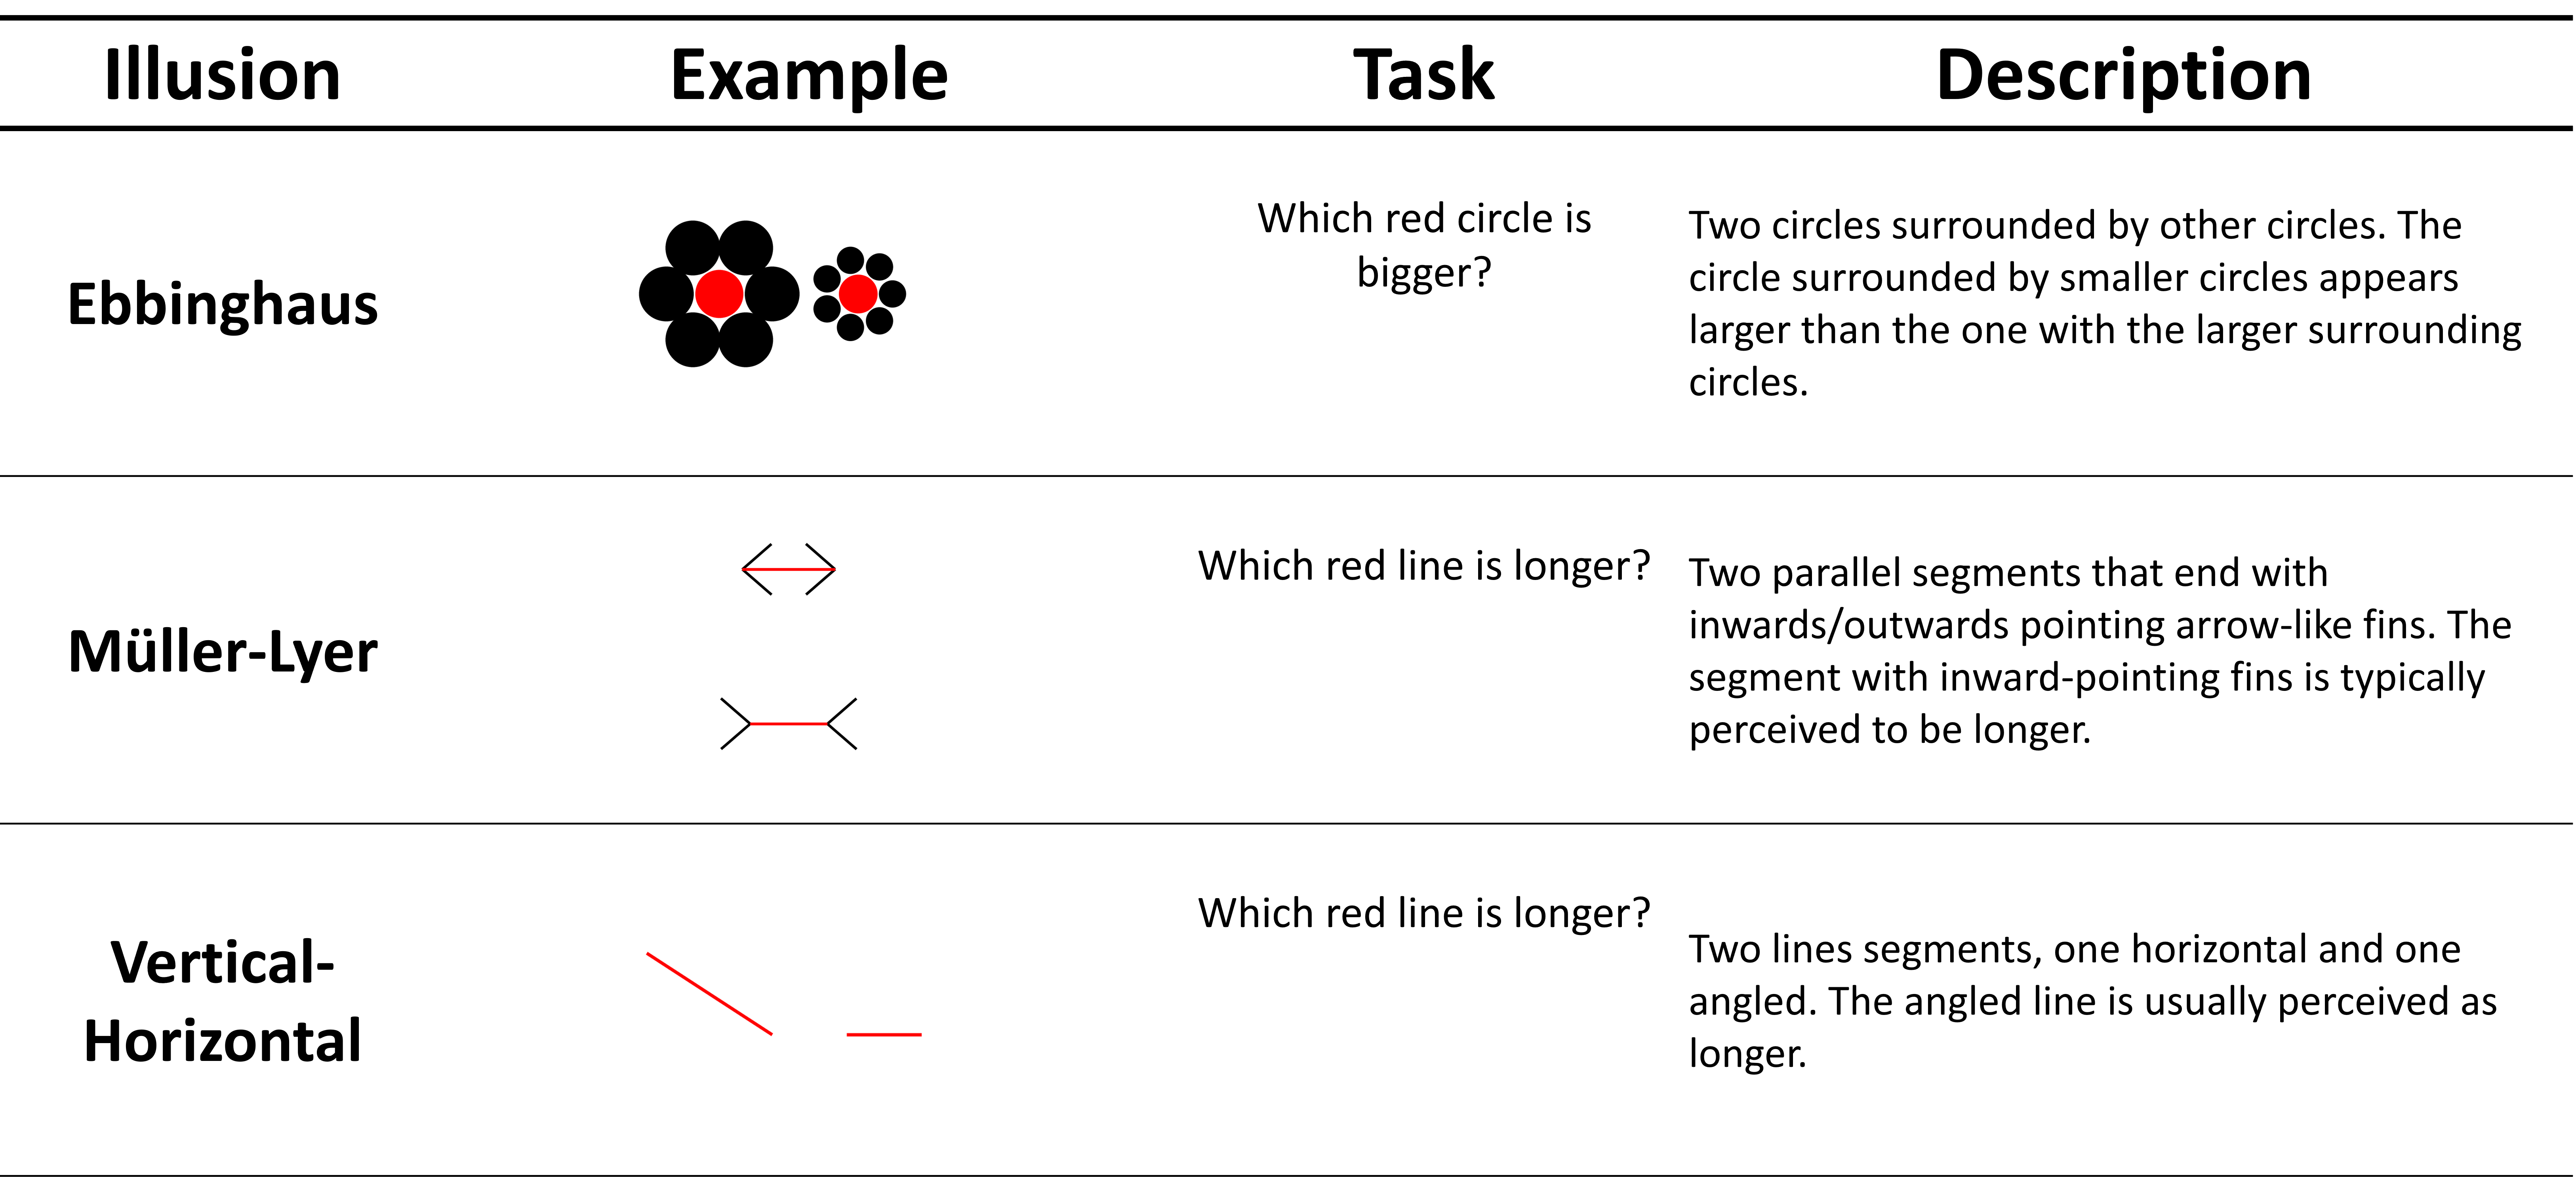
\includegraphics[width=1\linewidth,height=\textheight,keepaspectratio]{img/IllusionTable.jpg}

}

\end{figure}%

The procedure encompassed 2 sets of 80 trials for each illusion type,
preceded by a practice trial for each illusion. Each set included, in a
random order, the 3 blocks of illusion types, in which trials were
separated by a fixation cross, temporally (uniformly sampled duration of
500 - 1000ms) and spatially jittered (around the centre of the screen in
a radius of a 1 cm) to attenuate its potential usefulness as a reference
point. After each illusion type block, an arbitrary score was presented
(computed as a scaled Inverse Efficiency Score) as a gamification
mechanism to increase motivation to perform to the best of one's
abilities. To mitigate for the potential variability in the
speed/accuracy trade-off, the instructions emphasized with equal weight
to be fast and to avoid errors.

For each illusion type, two continuous dimensions were orthogonally
manipulated namely task difficulty and illusion strength, so that each
trial corresponds to a unique combination, providing an objectively
correct answer for each trial. The use of these manipulations allows
concise, standardised reporting of illusion parameters and ensures our
stimuli are fully reproducible (see \citeproc{ref-makowski2021}{Makowski
et al., 2021}).

Task difficulty corresponds to the difficulty of the perceptual decision
(e.g., if the task is to select the longest red line, task difficulty
corresponds to how the lines are objectively different). Illusion
strength corresponds to the degree to which the illusion elements (e.g.,
the black arrow lines in Müller-Lyer) are interfering with the
aforementioned task. Note that the illusion effect can be either
``incongruent'', making the task more difficult by biasing perceptual
decisions toward the incorrect response or ``congruent'', making the
task easier by biasing decisions toward the correct response (e.g., in
the Müller-Lyer illusion, if the outwards-facing arrowheads are placed
on the longer line, identifying which line is the longest becomes
easier). Participants responded with a key arrow (left vs.~right; or up
vs.~down), and their reaction time (RT) and accuracy were recorded.

Visual illusion sensitivity was measured as the average error rate in
the incongruent condition, and separately for the 3 illusion types.
Although the error rate is arguably a crude score, which does not take
into account the effect of varying illusion strength, the interaction
with task difficulty and the possible adjustments in response strategy
(speed-accuracy trade off), it is also the most simple and easy to
reproduce, hence its usage as our primary outcome for the current
registered report. As a secondary exploratory outcome, the Inverse
Efficiency Score {[}IES; Townsend and Ashby
(\citeproc{ref-townsend2014methods}{2014}){]} was computed. This metric
incorporates both speed and accuracy by dividing the mean reaction time
of correct responses by the proportion of correct responses, separately
for each illusion.

The two sets of 3 illusion blocks were separated by 2 short
questionnaires acting as a break, namely the IPIP-6
(\citeproc{ref-sibley2011mini}{{Sibley et al.}, 2011}), measuring 6
personality traits with 24 analogue scales items, and the PID-5
(\citeproc{ref-krueger2011}{Krueger et al., 2011}), measuring 5
maladaptive personality traits with 25 Likert scales items. These
questionnaires were included as a way of providing a break between the
two cognitively taxing blocks and maintain paradigmatic consistency with
previous studies (\citeproc{ref-makowski2023}{Makowski et al., 2023}).
Additionally, the psychoticism subscale of the PID-5 was used to examine
the correlation between maladaptive traits and illusion sensitivity,
evaluating the existence of the link proposed in previous studies
(\citeproc{ref-costa2023}{Costa et al., 2023}).

\subsection{Data Analysis}\label{data-analysis}

The phenomenological control scale \textbf{included} several attention
checks to identify problematic participants. The task \textbf{consisted}
of various auditory and visual exercises; at the outset, participants
\textbf{heard} a voice say ``Hello'' and \textbf{were} asked to select
the corresponding phrase from multiple options (i.e., ``Hello'',
``Goodbye'', ``How are you'', ``Thank you''). Selecting an incorrect
response \textbf{indicated} inattention to auditory stimuli. In a
subsequent exercise, participants \textbf{were} instructed: ``Open your
eyes. You will see only two balls on the screen\ldots{} just two
balls''. However, three differently coloured balls \textbf{were}
displayed. If a participant \textbf{selected} the response ``No Balls
Were Presented'', it \textbf{suggested} they failed to attend to both
the auditory instruction and the visual stimuli. In another task,
participants \textbf{were} instructed to press the spacebar six times.
Pressing it fewer than five times within the allotted time
\textbf{indicated} a failure to follow the auditory instructions.
Participants who \textbf{failed} any one of these \textbf{were to be}
excluded from further analysis \textbf{(see Deviations From
Registration)}. Finally, the reliability of the PCS \textbf{was}
assessed by computing Cronbach's alpha of its items
(\citeproc{ref-cronbach1951coefficient}{Cronbach, 1951}).

Outliers in the Illusion Game \textbf{were} identified based on
participants' performance. Specifically, any participant exhibiting an
error rate greater than 45\% for any illusion type \textbf{was}
considered to be responding at chance level (i.e., randomly) and flagged
accordingly. If this level of performance \textbf{occurred} in the first
block, the entire participant \textbf{was} excluded from analysis, as it
suggests a failure to properly engage with the task. However, if the
elevated error rate \textbf{was} observed only in the second block, this
\textbf{was} interpreted as a loss of engagement or motivation (e.g.,
boredom due to task repetition). In such cases, only the second block
\textbf{was} discarded, allowing for estimation of illusion sensitivity
based on the valid data from the first block, albeit with reduced
precision. To mitigate the risk of confounding effects driven by extreme
speed or accuracy strategies, participants whose \textbf{mean RT was
slower than} the group average (RT \textgreater{} 4 SD above the mean,
based on \citeproc{ref-makowski2023}{Makowski et al., 2023})
\textbf{were} excluded from the analysis. After removing problematic
participants and trials, the outcome measures (PC and VI sensitivity
scores) \textbf{were} computed.

To assess whether the illusions functioned as expected, stimuli
\textbf{were} categorized into three groups: Strong Illusion Strength \&
Incongruent, Mild Illusion Strength \& Incongruent, and Congruent. The
two outcome measures---error rate and IES---\textbf{were} computed
separately for each illusion and each illusion strength group. To
evaluate differences between these conditions, two Bayesian t-tests
\textbf{were} conducted: one comparing the Congruent and Mild
conditions, and the other comparing the Mild and Strong conditions.
\textbf{Evidence (\(BF_{10} > 3\)) for} differences in either IES or
error rate across these comparisons \textbf{was} taken as evidence that
the illusions operated as intended.

Next, to determine whether the Mild and Strong Illusion Strength groups
\textbf{could} be collapsed for further analysis, Bayesian correlations
\textbf{were} computed between them for each illusion and outcome
measure. If these correlations \textbf{were} sufficiently high (r
\textgreater{} .50, \citeproc{ref-cohen2013statistical}{Cohen, 2013}),
the groups \textbf{were} collapsed and outcomes recomputed across all
relevant trials (i.e., by averaging across these groups). If not, the
groups \textbf{were} analysed separately. This step \textbf{was}
necessary because reaction time may not have a linear relationship with
illusion strength (\citeproc{ref-makowski2023}{Makowski et al., 2023}),
and collapsing the data without this check may obscure meaningful
differences. Finally, reliability analyses \textbf{were} conducted on
all resulting indices, with Cronbach's alpha used to evaluate internal
consistency across the three illusion types.

Bayesian correlations \textbf{were} then computed between PCS and
illusion sensitivity scores - with the resulting IES and error rate
indices. Following Lush et al. (\citeproc{ref-lush2022}{2022}), we
\textbf{expected} to collect evidence against (\(BF_{10} \leq 1/3\)) a
relationship between PCS and VI sensitivity. Additionally, Bayesian
correlations \textbf{were} computed between maladaptive trait facets and
illusion sensitivity scores. Based on prior research
(\citeproc{ref-makowski2023}{Makowski et al., 2023}), we
\textbf{expected} to find evidence (\(BF_{10} > 3\)) supporting a
\textbf{(negative)} relationship between the psychoticism facet of the
PID-5 and illusion sensitivity. \textbf{Bayes factors between 1/3 and 3
were interpreted as inconclusive.}

All Bayesian analyses \textbf{were} conducted using the
\emph{BayesFactor} package (\citeproc{ref-BayesFactor}{Morey \& Rouder,
2024}). For correlations, a medium shifted beta prior \textbf{was}
applied (r-scale parameter set to 1/3), as recommended by Morey and
Rouder (\citeproc{ref-morey2018baysefactor}{2018}), providing a balanced
approach to estimating effect sizes, without placing undue weight on
larger effect sizes or artificially inflating evidence for the null
hypothesis. For t-tests, the \emph{ttestBF} function \textbf{was} used
with a medium Cauchy prior on the standardised effect size (r-scale =
√2⁄2), corresponding to the default for independent samples.

Data analysis \textbf{was} carried out using R, using \emph{tidyverse}
(\citeproc{ref-tidyverse}{Wickham et al., 2019}) and \emph{easystats}
(\citeproc{ref-parameters}{Lüdecke et al., 2020},
\citeproc{ref-easystats}{2022}; \citeproc{ref-bayestestR}{Makowski et
al., 2019}, \citeproc{ref-correlation}{2022};
\citeproc{ref-datawizard}{Patil et al., 2022}). The analysis script and
additional information are available at
\textbf{https://github.com/RealityBending/IllusionGamePhenomenologicalControl}.
\textbf{Departures from this registered plan are reported in the Results
as deviations.} \textbf{Their combined and individual effects on the
results were evaluated in sensitivity analyses (Table S1).}

\section{Results}\label{results}

\subsection{Data Exclusion}\label{data-exclusion}

\subsubsection{Registered Exclusions}\label{registered-exclusions}

\textbf{Of the 500 recruited participants, 19 failed the first two PCS
attention checks (10 did not report hearing ``Hello''; 9 reported that
no balls were presented), and 189 failed the space bar check, 181 of
whom had passed the first two checks (see Deviations From Registration).
Of the 300 participants who passed all three checks, in line with the
registered protocol, 4 participants with an error rate above 45\% for
any illusion type in the first block were fully excluded, 3 participants
exceeding this threshold only in the second block had that block removed
(these participants were retained), and 1 participant whose mean RT
exceeded the group mean by more than 4 SD was fully excluded. This left
295 participants for the fully registered analysis. The full sequence of
exclusions is shown in Figure S1.}

\subsubsection{Deviations From
Registration}\label{deviations-from-registration}

\textbf{During analysis, we identified three issues that could affect
the validity of the registered exclusions: an attention check that was
failed by a disproportionate number of participants, a small number of
participants who appeared to have misunderstood the task instructions,
and trials with implausible response times.} \textbf{These are described
below and were addressed together in an unregistered analysis, used as a
sensitivity analysis (see Sensitivity Analyses).}

\paragraph{Phenomenological Control.}\label{phenomenological-control}

The registered protocol specified that participants failing any of
\textbf{three} attention checks in the PCS would be excluded.
\textbf{The first two checks were failed by 19 participants (3.8\%),
whereas the third one was failed by 189 participants (37.8\%). Most
failures (177 of 189) recorded no presses at all, which argues against
dropped key presses (which would produce partial counts). Most of these
participants (181 of 189) passed the other two checks, and in the sample
used for the sensitivity analyses (N = 468), the scores of participants
who failed the space bar check on the remaining PCS items were not lower
than those of participants who passed it (\emph{M} = 2.49 vs.~2.28;
\(BF_{10} = 2.90\)), suggesting that failures did not reflect general
inattention. Instead, the failure rate may reflect how the check was
implemented: although the auditory instruction, delivered with eyes
closed, stated that the ``PLEASE WAIT'' message would appear ``a little
later'', the screen appeared as soon as the recording ended (i.e., as
participants were told to open their eyes), disappeared after 10
seconds, and only recorded presses made while it was displayed.
Participants who were still reorienting after opening their eyes, or who
pressed during the instruction, would therefore have been recorded as
not pressing at all.}

\textbf{We therefore repeated the analyses without the space bar check
as part of the unregistered analysis. In this sample (the 481
participants who passed the first two PCS checks), the registered
Illusion Game criteria fully excluded 8 participants on the basis of
error rate and 5 on the basis of RT (none of whom were flagged by both
criteria), and removed the second block of 7 participants (who were
retained), leaving 468 participants.}

\paragraph{Illusion Game.}\label{illusion-game-1}

\subparagraph{Participant exclusions (per
illusion).}\label{participant-exclusions-per-illusion}

During data inspection, a \textbf{small number} of participants
\textbf{showed very high error rates in the congruent condition, where
the illusion makes the task easier and errors are typically rare. These
patterns are more consistent with a misunderstanding of the instructions
(e.g., selecting the smaller instead of the larger circle) than with
illusion sensitivity. In the unregistered analysis, participants whose
congruent error rate for a given illusion lay above the 97.5\% highest
density interval (HDI) of its distribution (computed after the removal
of extreme trials; see Trial exclusions) were therefore excluded from
the analyses of that illusion only (10 participants, 2.14\%, for each
illusion), leaving 458 participants per illusion.}

\subparagraph{Trial exclusions.}\label{trial-exclusions}

\textbf{The Stage 1 protocol referred to the removal of problematic
trials but did not specify a criterion. In the unregistered analysis,
trials with response times below 0.2 s or above 5 s were excluded as
implausible (\citeproc{ref-theriault2024}{Thériault et al., 2024}),
removing 864 trials (0.39\% of the data; 298 faster than 0.2 s and 566
slower than 5 s).}

\subsection{Manipulation Check}\label{manipulation-check}

Bayesian paired-samples \emph{t}-tests \textbf{in the registered
analysis (N = 295)} revealed extreme evidence for differences between
\textbf{adjacent} illusion strength conditions, with performance
decreasing as illusion strength increased across all illusion types and
outcome measures (\(BF_{10} > 1000\)). For all three illusions
(Ebbinghaus, Müller--Lyer, Vertical--Horizontal), error rates and IES
were \textbf{lower} in the Congruent relative to Mild condition, and
lower in the Mild relative to Strong condition, consistent with the
expected effect of illusion strength (see Table~\ref{tbl-tablemeans}).

\global\setlength{\Oldarrayrulewidth}{\arrayrulewidth}

\global\setlength{\Oldtabcolsep}{\tabcolsep}

\setlength{\tabcolsep}{2pt}

\renewcommand*{\arraystretch}{1.5}



\providecommand{\ascline}[3]{\noalign{\global\arrayrulewidth #1}\arrayrulecolor[HTML]{#2}\cline{#3}}

\begin{longtable}[c]{ccccccc}

\caption{\label{tbl-tablemeans}Mean and standard deviation of error rate
and IES for each illusion type and strength condition in the registered
analysis (N = 295). All differences between adjacent illusion strength
conditions showed extreme evidence (\(BF_{10} > 1000\)).}

\tabularnewline

\ascline{1.5pt}{666666}{1-7}

\multicolumn{1}{>{}l}{\advance\leftskip by 5.0pt\relax \advance\rightskip by 5.0pt\relax \textcolor[HTML]{000000}{\fontsize{11}{11}\selectfont{{\fontspec{Arial} Illusion}}}} & \multicolumn{1}{>{}l}{\advance\leftskip by 5.0pt\relax \advance\rightskip by 5.0pt\relax \textcolor[HTML]{000000}{\fontsize{11}{11}\selectfont{{\fontspec{Arial} Error\ Rate\ -\ Congruent}}}} & \multicolumn{1}{>{}l}{\advance\leftskip by 5.0pt\relax \advance\rightskip by 5.0pt\relax \textcolor[HTML]{000000}{\fontsize{11}{11}\selectfont{{\fontspec{Arial} Error\ Rate\ -\ Mild}}}} & \multicolumn{1}{>{}l}{\advance\leftskip by 5.0pt\relax \advance\rightskip by 5.0pt\relax \textcolor[HTML]{000000}{\fontsize{11}{11}\selectfont{{\fontspec{Arial} Error\ Rate\ -\ Strong}}}} & \multicolumn{1}{>{}l}{\advance\leftskip by 5.0pt\relax \advance\rightskip by 5.0pt\relax \textcolor[HTML]{000000}{\fontsize{11}{11}\selectfont{{\fontspec{Arial} IES\ -\ Congruent}}}} & \multicolumn{1}{>{}l}{\advance\leftskip by 5.0pt\relax \advance\rightskip by 5.0pt\relax \textcolor[HTML]{000000}{\fontsize{11}{11}\selectfont{{\fontspec{Arial} IES\ -\ Mild}}}} & \multicolumn{1}{>{}l}{\advance\leftskip by 5.0pt\relax \advance\rightskip by 5.0pt\relax \textcolor[HTML]{000000}{\fontsize{11}{11}\selectfont{{\fontspec{Arial} IES\ -\ Strong}}}} \\

\ascline{1.5pt}{666666}{1-7}\endfirsthead 

\ascline{1.5pt}{666666}{1-7}

\multicolumn{1}{>{}l}{\advance\leftskip by 5.0pt\relax \advance\rightskip by 5.0pt\relax \textcolor[HTML]{000000}{\fontsize{11}{11}\selectfont{{\fontspec{Arial} Illusion}}}} & \multicolumn{1}{>{}l}{\advance\leftskip by 5.0pt\relax \advance\rightskip by 5.0pt\relax \textcolor[HTML]{000000}{\fontsize{11}{11}\selectfont{{\fontspec{Arial} Error\ Rate\ -\ Congruent}}}} & \multicolumn{1}{>{}l}{\advance\leftskip by 5.0pt\relax \advance\rightskip by 5.0pt\relax \textcolor[HTML]{000000}{\fontsize{11}{11}\selectfont{{\fontspec{Arial} Error\ Rate\ -\ Mild}}}} & \multicolumn{1}{>{}l}{\advance\leftskip by 5.0pt\relax \advance\rightskip by 5.0pt\relax \textcolor[HTML]{000000}{\fontsize{11}{11}\selectfont{{\fontspec{Arial} Error\ Rate\ -\ Strong}}}} & \multicolumn{1}{>{}l}{\advance\leftskip by 5.0pt\relax \advance\rightskip by 5.0pt\relax \textcolor[HTML]{000000}{\fontsize{11}{11}\selectfont{{\fontspec{Arial} IES\ -\ Congruent}}}} & \multicolumn{1}{>{}l}{\advance\leftskip by 5.0pt\relax \advance\rightskip by 5.0pt\relax \textcolor[HTML]{000000}{\fontsize{11}{11}\selectfont{{\fontspec{Arial} IES\ -\ Mild}}}} & \multicolumn{1}{>{}l}{\advance\leftskip by 5.0pt\relax \advance\rightskip by 5.0pt\relax \textcolor[HTML]{000000}{\fontsize{11}{11}\selectfont{{\fontspec{Arial} IES\ -\ Strong}}}} \\

\ascline{1.5pt}{666666}{1-7}\endhead



\multicolumn{1}{>{}l}{\advance\leftskip by 5.0pt\relax \advance\rightskip by 5.0pt\relax \textcolor[HTML]{000000}{\fontsize{10}{10}\selectfont{{\fontspec{Arial} Ebbinghaus}}}} & \multicolumn{1}{>{}l}{\advance\leftskip by 5.0pt\relax \advance\rightskip by 5.0pt\relax \textcolor[HTML]{000000}{\fontsize{10}{10}\selectfont{{\fontspec{Arial} 4.01\%\ ±\ 7\%}}}} & \multicolumn{1}{>{}l}{\advance\leftskip by 5.0pt\relax \advance\rightskip by 5.0pt\relax \textcolor[HTML]{000000}{\fontsize{10}{10}\selectfont{{\fontspec{Arial} 15.57\%\ ±\ 9\%}}}} & \multicolumn{1}{>{}l}{\advance\leftskip by 5.0pt\relax \advance\rightskip by 5.0pt\relax \textcolor[HTML]{000000}{\fontsize{10}{10}\selectfont{{\fontspec{Arial} 40.85\%\ ±\ 17\%}}}} & \multicolumn{1}{>{}l}{\advance\leftskip by 5.0pt\relax \advance\rightskip by 5.0pt\relax \textcolor[HTML]{000000}{\fontsize{10}{10}\selectfont{{\fontspec{Arial} 0.81\ \ ±\ 0.29}}}} & \multicolumn{1}{>{}l}{\advance\leftskip by 5.0pt\relax \advance\rightskip by 5.0pt\relax \textcolor[HTML]{000000}{\fontsize{10}{10}\selectfont{{\fontspec{Arial} 1.05\ \ ±\ 0.42}}}} & \multicolumn{1}{>{}l}{\advance\leftskip by 5.0pt\relax \advance\rightskip by 5.0pt\relax \textcolor[HTML]{000000}{\fontsize{10}{10}\selectfont{{\fontspec{Arial} 2.05\ \ ±\ 3.09}}}} \\





\multicolumn{1}{>{}l}{\advance\leftskip by 5.0pt\relax \advance\rightskip by 5.0pt\relax \textcolor[HTML]{000000}{\fontsize{10}{10}\selectfont{{\fontspec{Arial} Müller-Lyer}}}} & \multicolumn{1}{>{}l}{\advance\leftskip by 5.0pt\relax \advance\rightskip by 5.0pt\relax \textcolor[HTML]{000000}{\fontsize{10}{10}\selectfont{{\fontspec{Arial} 1.02\%\ ±\ 2\%}}}} & \multicolumn{1}{>{}l}{\advance\leftskip by 5.0pt\relax \advance\rightskip by 5.0pt\relax \textcolor[HTML]{000000}{\fontsize{10}{10}\selectfont{{\fontspec{Arial} 24.95\%\ ±\ 7\%}}}} & \multicolumn{1}{>{}l}{\advance\leftskip by 5.0pt\relax \advance\rightskip by 5.0pt\relax \textcolor[HTML]{000000}{\fontsize{10}{10}\selectfont{{\fontspec{Arial} 61.38\%\ ±\ 13\%}}}} & \multicolumn{1}{>{}l}{\advance\leftskip by 5.0pt\relax \advance\rightskip by 5.0pt\relax \textcolor[HTML]{000000}{\fontsize{10}{10}\selectfont{{\fontspec{Arial} 0.65\ \ ±\ 0.16}}}} & \multicolumn{1}{>{}l}{\advance\leftskip by 5.0pt\relax \advance\rightskip by 5.0pt\relax \textcolor[HTML]{000000}{\fontsize{10}{10}\selectfont{{\fontspec{Arial} 1.12\ \ ±\ 0.31}}}} & \multicolumn{1}{>{}l}{\advance\leftskip by 5.0pt\relax \advance\rightskip by 5.0pt\relax \textcolor[HTML]{000000}{\fontsize{10}{10}\selectfont{{\fontspec{Arial} 2.81\ \ ±\ 1.25}}}} \\





\multicolumn{1}{>{}l}{\advance\leftskip by 5.0pt\relax \advance\rightskip by 5.0pt\relax \textcolor[HTML]{000000}{\fontsize{10}{10}\selectfont{{\fontspec{Arial} Vertical–Horizontal}}}} & \multicolumn{1}{>{}l}{\advance\leftskip by 5.0pt\relax \advance\rightskip by 5.0pt\relax \textcolor[HTML]{000000}{\fontsize{10}{10}\selectfont{{\fontspec{Arial} 2.98\%\ ±\ 3\%}}}} & \multicolumn{1}{>{}l}{\advance\leftskip by 5.0pt\relax \advance\rightskip by 5.0pt\relax \textcolor[HTML]{000000}{\fontsize{10}{10}\selectfont{{\fontspec{Arial} 19.44\%\ ±\ 10\%}}}} & \multicolumn{1}{>{}l}{\advance\leftskip by 5.0pt\relax \advance\rightskip by 5.0pt\relax \textcolor[HTML]{000000}{\fontsize{10}{10}\selectfont{{\fontspec{Arial} 52.64\%\ ±\ 17\%}}}} & \multicolumn{1}{>{}l}{\advance\leftskip by 5.0pt\relax \advance\rightskip by 5.0pt\relax \textcolor[HTML]{000000}{\fontsize{10}{10}\selectfont{{\fontspec{Arial} 0.69\ \ ±\ 0.21}}}} & \multicolumn{1}{>{}l}{\advance\leftskip by 5.0pt\relax \advance\rightskip by 5.0pt\relax \textcolor[HTML]{000000}{\fontsize{10}{10}\selectfont{{\fontspec{Arial} 1.05\ \ ±\ 0.35}}}} & \multicolumn{1}{>{}l}{\advance\leftskip by 5.0pt\relax \advance\rightskip by 5.0pt\relax \textcolor[HTML]{000000}{\fontsize{10}{10}\selectfont{{\fontspec{Arial} 2.43\ \ ±\ 1.72}}}} \\

\ascline{1.5pt}{666666}{1-7}


\end{longtable}

\arrayrulecolor[HTML]{000000}

\global\setlength{\arrayrulewidth}{\Oldarrayrulewidth}

\global\setlength{\tabcolsep}{\Oldtabcolsep}

\renewcommand*{\arraystretch}{1}

\subsection{Score Consistency}\label{score-consistency}

The 10 items forming the PCS score yielded acceptable consistency
(\(\alpha = 0.78\)). \textbf{PCS scores (possible range 0--5) had a mean
of 2.16 (\emph{SD} = 0.80, range: 0.00--4.20), and psychoticism scores
(possible range 0-3) a mean of 0.48 (\emph{SD} = 0.40, range:
0.00--1.80), with a positively skewed distribution (skewness = 0.85;
Figure S2).}

For the illusion scores, the registered plan was to first evaluate
\textbf{whether the Mild and Strong illusion strength conditions could
be collapsed, based on the correlation between them for each illusion
and outcome (collapsed if r \textgreater{} .50; Table S2)}.
\textbf{Error rates were collapsed for all three illusions (Müller-Lyer:
\emph{r} = .67; Ebbinghaus: \emph{r} = .76; Vertical--Horizontal:
\emph{r} = .72).} \textbf{IES were collapsed for the Müller-Lyer
(\emph{r} = .55) and Ebbinghaus illusions (\emph{r} = .54), but analysed
separately for the Vertical--Horizontal illusion (\emph{r} = .43).}
\textbf{Analyses with Mild and Strong kept separate for all scores are
reported as exploratory analyses.}

Consistency analyses between the 3 illusions were conducted as
registered, using Cronbach's alpha. Error rate consistency was low
(Mild: \textbf{\(\alpha = .33\)}; Strong: \textbf{\(\alpha = .06\)};
collapsed: \textbf{\(\alpha = .19\)}), whereas IES \textbf{consistency}
was mixed (Mild: \(\alpha = .83\); Strong: \(\alpha = .17\);
\textbf{collapsed: \(\alpha = .74\)}), overall providing no evidence for
combining the scores of the 3 illusions.

\subsection{Correlations}\label{correlations}

\subsubsection{Registered Analysis}\label{registered-analysis}

Bayesian correlations were conducted to assess the relationship between
illusion sensitivity (\textbf{error rate as the primary outcome and IES
as the secondary outcome}) and both PCS scores and the psychoticism
facet of the PID-5. \textbf{All registered tests are reported in
Table~\ref{tbl-correlations} and displayed in Figure~\ref{fig-corr}.}

\textbf{Of the 14 registered tests, 10 met the threshold for evidence
for the null (\(BF_{10} \leq 1/3\)), 4 were inconclusive, and none
supported a relationship.} \textbf{For the primary outcome (error rate),
the correlation between PCS and illusion sensitivity provided evidence
for the null for the Müller-Lyer (\(\rho = 0.05\), \(BF_{10} = 0.19\))
and Ebbinghaus illusions (\(\rho = 0.02\), \(BF_{10} = 0.14\)), and was
inconclusive for the Vertical-Horizontal illusion (\(\rho = 0.08\),
\(BF_{10} = 0.38\)).} \textbf{For the secondary outcome (IES), 3 of the
4 PCS tests supported the null and 1 was inconclusive (Müller-Lyer,
\(BF_{10} = 0.45\)).}

\textbf{The correlations between psychoticism and error rates all
supported the null (\(BF_{10} = 0.14\)--\(0.17\)), as did 2 of the 4 IES
tests, while the other 2 were inconclusive (\(BF_{10} = 0.40\) and
\(BF_{10} = 0.92\)).} \textbf{None of the registered tests therefore
supported the hypothesised negative association between psychoticism and
illusion sensitivity.}

\begin{table}

{\caption{{Registered Bayesian correlations between illusion sensitivity
and dispositional traits (registered analysis, N = 295). Mild and Strong
conditions were collapsed (Mild + Strong) or analysed separately
according to the registered decision rule. ρ = posterior median with
95\% credible interval. Evidence: Null = \(BF_{10} \leq 1/3\);
Inconclusive = \(1/3 < BF_{10} < 3\); Relationship =
\(BF_{10} \geq 3\).}{\label{tbl-correlations}}}
\vspace{-20pt}}

\global\setlength{\Oldarrayrulewidth}{\arrayrulewidth}

\global\setlength{\Oldtabcolsep}{\tabcolsep}

\setlength{\tabcolsep}{2pt}

\renewcommand*{\arraystretch}{1.5}



\providecommand{\ascline}[3]{\noalign{\global\arrayrulewidth #1}\arrayrulecolor[HTML]{#2}\cline{#3}}

\begin{longtable*}[c]{ccccccc}



\ascline{1.5pt}{666666}{1-7}

\multicolumn{1}{>{}l}{\advance\leftskip by 5.0pt\relax \advance\rightskip by 5.0pt\relax \textcolor[HTML]{000000}{\fontsize{9}{9}\selectfont{{\fontspec{Arial} Trait}}}} & \multicolumn{1}{>{}l}{\advance\leftskip by 5.0pt\relax \advance\rightskip by 5.0pt\relax \textcolor[HTML]{000000}{\fontsize{9}{9}\selectfont{{\fontspec{Arial} Outcome}}}} & \multicolumn{1}{>{}l}{\advance\leftskip by 5.0pt\relax \advance\rightskip by 5.0pt\relax \textcolor[HTML]{000000}{\fontsize{9}{9}\selectfont{{\fontspec{Arial} Illusion}}}} & \multicolumn{1}{>{}l}{\advance\leftskip by 5.0pt\relax \advance\rightskip by 5.0pt\relax \textcolor[HTML]{000000}{\fontsize{9}{9}\selectfont{{\fontspec{Arial} Condition}}}} & \multicolumn{1}{>{}l}{\advance\leftskip by 5.0pt\relax \advance\rightskip by 5.0pt\relax \textcolor[HTML]{000000}{\fontsize{9}{9}\selectfont{{\fontspec{Arial} ρ\ [95\%\ CI]}}}} & \multicolumn{1}{>{}l}{\advance\leftskip by 5.0pt\relax \advance\rightskip by 5.0pt\relax \textcolor[HTML]{000000}{\fontsize{9}{9}\selectfont{{\fontspec{Arial} BF₁₀}}}} & \multicolumn{1}{>{}l}{\advance\leftskip by 5.0pt\relax \advance\rightskip by 5.0pt\relax \textcolor[HTML]{000000}{\fontsize{9}{9}\selectfont{{\fontspec{Arial} Evidence}}}} \\

\ascline{1.5pt}{666666}{1-7}\endfirsthead 

\ascline{1.5pt}{666666}{1-7}

\multicolumn{1}{>{}l}{\advance\leftskip by 5.0pt\relax \advance\rightskip by 5.0pt\relax \textcolor[HTML]{000000}{\fontsize{9}{9}\selectfont{{\fontspec{Arial} Trait}}}} & \multicolumn{1}{>{}l}{\advance\leftskip by 5.0pt\relax \advance\rightskip by 5.0pt\relax \textcolor[HTML]{000000}{\fontsize{9}{9}\selectfont{{\fontspec{Arial} Outcome}}}} & \multicolumn{1}{>{}l}{\advance\leftskip by 5.0pt\relax \advance\rightskip by 5.0pt\relax \textcolor[HTML]{000000}{\fontsize{9}{9}\selectfont{{\fontspec{Arial} Illusion}}}} & \multicolumn{1}{>{}l}{\advance\leftskip by 5.0pt\relax \advance\rightskip by 5.0pt\relax \textcolor[HTML]{000000}{\fontsize{9}{9}\selectfont{{\fontspec{Arial} Condition}}}} & \multicolumn{1}{>{}l}{\advance\leftskip by 5.0pt\relax \advance\rightskip by 5.0pt\relax \textcolor[HTML]{000000}{\fontsize{9}{9}\selectfont{{\fontspec{Arial} ρ\ [95\%\ CI]}}}} & \multicolumn{1}{>{}l}{\advance\leftskip by 5.0pt\relax \advance\rightskip by 5.0pt\relax \textcolor[HTML]{000000}{\fontsize{9}{9}\selectfont{{\fontspec{Arial} BF₁₀}}}} & \multicolumn{1}{>{}l}{\advance\leftskip by 5.0pt\relax \advance\rightskip by 5.0pt\relax \textcolor[HTML]{000000}{\fontsize{9}{9}\selectfont{{\fontspec{Arial} Evidence}}}} \\

\ascline{1.5pt}{666666}{1-7}\endhead



\multicolumn{1}{>{}l}{\advance\leftskip by 5.0pt\relax \advance\rightskip by 5.0pt\relax \textcolor[HTML]{000000}{\fontsize{9}{9}\selectfont{{\fontspec{Arial} PCS}}}} & \multicolumn{1}{>{}l}{\advance\leftskip by 5.0pt\relax \advance\rightskip by 5.0pt\relax \textcolor[HTML]{000000}{\fontsize{9}{9}\selectfont{{\fontspec{Arial} Error\ rate\ (primary)}}}} & \multicolumn{1}{>{}l}{\advance\leftskip by 5.0pt\relax \advance\rightskip by 5.0pt\relax \textcolor[HTML]{000000}{\fontsize{9}{9}\selectfont{{\fontspec{Arial} Ebbinghaus}}}} & \multicolumn{1}{>{}l}{\advance\leftskip by 5.0pt\relax \advance\rightskip by 5.0pt\relax \textcolor[HTML]{000000}{\fontsize{9}{9}\selectfont{{\fontspec{Arial} Mild\ +\ Strong}}}} & \multicolumn{1}{>{}l}{\advance\leftskip by 5.0pt\relax \advance\rightskip by 5.0pt\relax \textcolor[HTML]{000000}{\fontsize{9}{9}\selectfont{{\fontspec{Arial} 0.02\ [-0.10,\ 0.13]}}}} & \multicolumn{1}{>{}l}{\advance\leftskip by 5.0pt\relax \advance\rightskip by 5.0pt\relax \textcolor[HTML]{000000}{\fontsize{9}{9}\selectfont{{\fontspec{Arial} 0.14}}}} & \multicolumn{1}{>{}l}{\advance\leftskip by 5.0pt\relax \advance\rightskip by 5.0pt\relax \textcolor[HTML]{000000}{\fontsize{9}{9}\selectfont{{\fontspec{Arial} Null}}}} \\





\multicolumn{1}{>{}l}{\advance\leftskip by 5.0pt\relax \advance\rightskip by 5.0pt\relax \textcolor[HTML]{000000}{\fontsize{9}{9}\selectfont{{\fontspec{Arial} PCS}}}} & \multicolumn{1}{>{}l}{\advance\leftskip by 5.0pt\relax \advance\rightskip by 5.0pt\relax \textcolor[HTML]{000000}{\fontsize{9}{9}\selectfont{{\fontspec{Arial} Error\ rate\ (primary)}}}} & \multicolumn{1}{>{}l}{\advance\leftskip by 5.0pt\relax \advance\rightskip by 5.0pt\relax \textcolor[HTML]{000000}{\fontsize{9}{9}\selectfont{{\fontspec{Arial} Müller-Lyer}}}} & \multicolumn{1}{>{}l}{\advance\leftskip by 5.0pt\relax \advance\rightskip by 5.0pt\relax \textcolor[HTML]{000000}{\fontsize{9}{9}\selectfont{{\fontspec{Arial} Mild\ +\ Strong}}}} & \multicolumn{1}{>{}l}{\advance\leftskip by 5.0pt\relax \advance\rightskip by 5.0pt\relax \textcolor[HTML]{000000}{\fontsize{9}{9}\selectfont{{\fontspec{Arial} 0.04\ [-0.07,\ 0.16]}}}} & \multicolumn{1}{>{}l}{\advance\leftskip by 5.0pt\relax \advance\rightskip by 5.0pt\relax \textcolor[HTML]{000000}{\fontsize{9}{9}\selectfont{{\fontspec{Arial} 0.19}}}} & \multicolumn{1}{>{}l}{\advance\leftskip by 5.0pt\relax \advance\rightskip by 5.0pt\relax \textcolor[HTML]{000000}{\fontsize{9}{9}\selectfont{{\fontspec{Arial} Null}}}} \\





\multicolumn{1}{>{}l}{\advance\leftskip by 5.0pt\relax \advance\rightskip by 5.0pt\relax \textcolor[HTML]{000000}{\fontsize{9}{9}\selectfont{{\fontspec{Arial} PCS}}}} & \multicolumn{1}{>{}l}{\advance\leftskip by 5.0pt\relax \advance\rightskip by 5.0pt\relax \textcolor[HTML]{000000}{\fontsize{9}{9}\selectfont{{\fontspec{Arial} Error\ rate\ (primary)}}}} & \multicolumn{1}{>{}l}{\advance\leftskip by 5.0pt\relax \advance\rightskip by 5.0pt\relax \textcolor[HTML]{000000}{\fontsize{9}{9}\selectfont{{\fontspec{Arial} Vertical–Horizontal}}}} & \multicolumn{1}{>{}l}{\advance\leftskip by 5.0pt\relax \advance\rightskip by 5.0pt\relax \textcolor[HTML]{000000}{\fontsize{9}{9}\selectfont{{\fontspec{Arial} Mild\ +\ Strong}}}} & \multicolumn{1}{>{}l}{\advance\leftskip by 5.0pt\relax \advance\rightskip by 5.0pt\relax \textcolor[HTML]{000000}{\fontsize{9}{9}\selectfont{{\fontspec{Arial} 0.08\ [-0.03,\ 0.19]}}}} & \multicolumn{1}{>{}l}{\advance\leftskip by 5.0pt\relax \advance\rightskip by 5.0pt\relax \textcolor[HTML]{000000}{\fontsize{9}{9}\selectfont{{\fontspec{Arial} 0.38}}}} & \multicolumn{1}{>{}l}{\advance\leftskip by 5.0pt\relax \advance\rightskip by 5.0pt\relax \textcolor[HTML]{000000}{\fontsize{9}{9}\selectfont{{\fontspec{Arial} Inconclusive}}}} \\





\multicolumn{1}{>{}l}{\advance\leftskip by 5.0pt\relax \advance\rightskip by 5.0pt\relax \textcolor[HTML]{000000}{\fontsize{9}{9}\selectfont{{\fontspec{Arial} PCS}}}} & \multicolumn{1}{>{}l}{\advance\leftskip by 5.0pt\relax \advance\rightskip by 5.0pt\relax \textcolor[HTML]{000000}{\fontsize{9}{9}\selectfont{{\fontspec{Arial} IES\ (secondary)}}}} & \multicolumn{1}{>{}l}{\advance\leftskip by 5.0pt\relax \advance\rightskip by 5.0pt\relax \textcolor[HTML]{000000}{\fontsize{9}{9}\selectfont{{\fontspec{Arial} Ebbinghaus}}}} & \multicolumn{1}{>{}l}{\advance\leftskip by 5.0pt\relax \advance\rightskip by 5.0pt\relax \textcolor[HTML]{000000}{\fontsize{9}{9}\selectfont{{\fontspec{Arial} Mild\ +\ Strong}}}} & \multicolumn{1}{>{}l}{\advance\leftskip by 5.0pt\relax \advance\rightskip by 5.0pt\relax \textcolor[HTML]{000000}{\fontsize{9}{9}\selectfont{{\fontspec{Arial} 0.03\ [-0.07,\ 0.15]}}}} & \multicolumn{1}{>{}l}{\advance\leftskip by 5.0pt\relax \advance\rightskip by 5.0pt\relax \textcolor[HTML]{000000}{\fontsize{9}{9}\selectfont{{\fontspec{Arial} 0.16}}}} & \multicolumn{1}{>{}l}{\advance\leftskip by 5.0pt\relax \advance\rightskip by 5.0pt\relax \textcolor[HTML]{000000}{\fontsize{9}{9}\selectfont{{\fontspec{Arial} Null}}}} \\





\multicolumn{1}{>{}l}{\advance\leftskip by 5.0pt\relax \advance\rightskip by 5.0pt\relax \textcolor[HTML]{000000}{\fontsize{9}{9}\selectfont{{\fontspec{Arial} PCS}}}} & \multicolumn{1}{>{}l}{\advance\leftskip by 5.0pt\relax \advance\rightskip by 5.0pt\relax \textcolor[HTML]{000000}{\fontsize{9}{9}\selectfont{{\fontspec{Arial} IES\ (secondary)}}}} & \multicolumn{1}{>{}l}{\advance\leftskip by 5.0pt\relax \advance\rightskip by 5.0pt\relax \textcolor[HTML]{000000}{\fontsize{9}{9}\selectfont{{\fontspec{Arial} Müller-Lyer}}}} & \multicolumn{1}{>{}l}{\advance\leftskip by 5.0pt\relax \advance\rightskip by 5.0pt\relax \textcolor[HTML]{000000}{\fontsize{9}{9}\selectfont{{\fontspec{Arial} Mild\ +\ Strong}}}} & \multicolumn{1}{>{}l}{\advance\leftskip by 5.0pt\relax \advance\rightskip by 5.0pt\relax \textcolor[HTML]{000000}{\fontsize{9}{9}\selectfont{{\fontspec{Arial} 0.09\ [-0.03,\ 0.20]}}}} & \multicolumn{1}{>{}l}{\advance\leftskip by 5.0pt\relax \advance\rightskip by 5.0pt\relax \textcolor[HTML]{000000}{\fontsize{9}{9}\selectfont{{\fontspec{Arial} 0.45}}}} & \multicolumn{1}{>{}l}{\advance\leftskip by 5.0pt\relax \advance\rightskip by 5.0pt\relax \textcolor[HTML]{000000}{\fontsize{9}{9}\selectfont{{\fontspec{Arial} Inconclusive}}}} \\





\multicolumn{1}{>{}l}{\advance\leftskip by 5.0pt\relax \advance\rightskip by 5.0pt\relax \textcolor[HTML]{000000}{\fontsize{9}{9}\selectfont{{\fontspec{Arial} PCS}}}} & \multicolumn{1}{>{}l}{\advance\leftskip by 5.0pt\relax \advance\rightskip by 5.0pt\relax \textcolor[HTML]{000000}{\fontsize{9}{9}\selectfont{{\fontspec{Arial} IES\ (secondary)}}}} & \multicolumn{1}{>{}l}{\advance\leftskip by 5.0pt\relax \advance\rightskip by 5.0pt\relax \textcolor[HTML]{000000}{\fontsize{9}{9}\selectfont{{\fontspec{Arial} Vertical–Horizontal}}}} & \multicolumn{1}{>{}l}{\advance\leftskip by 5.0pt\relax \advance\rightskip by 5.0pt\relax \textcolor[HTML]{000000}{\fontsize{9}{9}\selectfont{{\fontspec{Arial} Mild}}}} & \multicolumn{1}{>{}l}{\advance\leftskip by 5.0pt\relax \advance\rightskip by 5.0pt\relax \textcolor[HTML]{000000}{\fontsize{9}{9}\selectfont{{\fontspec{Arial} 0.07\ [-0.04,\ 0.18]}}}} & \multicolumn{1}{>{}l}{\advance\leftskip by 5.0pt\relax \advance\rightskip by 5.0pt\relax \textcolor[HTML]{000000}{\fontsize{9}{9}\selectfont{{\fontspec{Arial} 0.32}}}} & \multicolumn{1}{>{}l}{\advance\leftskip by 5.0pt\relax \advance\rightskip by 5.0pt\relax \textcolor[HTML]{000000}{\fontsize{9}{9}\selectfont{{\fontspec{Arial} Null}}}} \\





\multicolumn{1}{>{}l}{\advance\leftskip by 5.0pt\relax \advance\rightskip by 5.0pt\relax \textcolor[HTML]{000000}{\fontsize{9}{9}\selectfont{{\fontspec{Arial} PCS}}}} & \multicolumn{1}{>{}l}{\advance\leftskip by 5.0pt\relax \advance\rightskip by 5.0pt\relax \textcolor[HTML]{000000}{\fontsize{9}{9}\selectfont{{\fontspec{Arial} IES\ (secondary)}}}} & \multicolumn{1}{>{}l}{\advance\leftskip by 5.0pt\relax \advance\rightskip by 5.0pt\relax \textcolor[HTML]{000000}{\fontsize{9}{9}\selectfont{{\fontspec{Arial} Vertical–Horizontal}}}} & \multicolumn{1}{>{}l}{\advance\leftskip by 5.0pt\relax \advance\rightskip by 5.0pt\relax \textcolor[HTML]{000000}{\fontsize{9}{9}\selectfont{{\fontspec{Arial} Strong}}}} & \multicolumn{1}{>{}l}{\advance\leftskip by 5.0pt\relax \advance\rightskip by 5.0pt\relax \textcolor[HTML]{000000}{\fontsize{9}{9}\selectfont{{\fontspec{Arial} 0.02\ [-0.09,\ 0.13]}}}} & \multicolumn{1}{>{}l}{\advance\leftskip by 5.0pt\relax \advance\rightskip by 5.0pt\relax \textcolor[HTML]{000000}{\fontsize{9}{9}\selectfont{{\fontspec{Arial} 0.15}}}} & \multicolumn{1}{>{}l}{\advance\leftskip by 5.0pt\relax \advance\rightskip by 5.0pt\relax \textcolor[HTML]{000000}{\fontsize{9}{9}\selectfont{{\fontspec{Arial} Null}}}} \\





\multicolumn{1}{>{}l}{\advance\leftskip by 5.0pt\relax \advance\rightskip by 5.0pt\relax \textcolor[HTML]{000000}{\fontsize{9}{9}\selectfont{{\fontspec{Arial} Psychoticism}}}} & \multicolumn{1}{>{}l}{\advance\leftskip by 5.0pt\relax \advance\rightskip by 5.0pt\relax \textcolor[HTML]{000000}{\fontsize{9}{9}\selectfont{{\fontspec{Arial} Error\ rate\ (primary)}}}} & \multicolumn{1}{>{}l}{\advance\leftskip by 5.0pt\relax \advance\rightskip by 5.0pt\relax \textcolor[HTML]{000000}{\fontsize{9}{9}\selectfont{{\fontspec{Arial} Ebbinghaus}}}} & \multicolumn{1}{>{}l}{\advance\leftskip by 5.0pt\relax \advance\rightskip by 5.0pt\relax \textcolor[HTML]{000000}{\fontsize{9}{9}\selectfont{{\fontspec{Arial} Mild\ +\ Strong}}}} & \multicolumn{1}{>{}l}{\advance\leftskip by 5.0pt\relax \advance\rightskip by 5.0pt\relax \textcolor[HTML]{000000}{\fontsize{9}{9}\selectfont{{\fontspec{Arial} 0.04\ [-0.08,\ 0.15]}}}} & \multicolumn{1}{>{}l}{\advance\leftskip by 5.0pt\relax \advance\rightskip by 5.0pt\relax \textcolor[HTML]{000000}{\fontsize{9}{9}\selectfont{{\fontspec{Arial} 0.16}}}} & \multicolumn{1}{>{}l}{\advance\leftskip by 5.0pt\relax \advance\rightskip by 5.0pt\relax \textcolor[HTML]{000000}{\fontsize{9}{9}\selectfont{{\fontspec{Arial} Null}}}} \\





\multicolumn{1}{>{}l}{\advance\leftskip by 5.0pt\relax \advance\rightskip by 5.0pt\relax \textcolor[HTML]{000000}{\fontsize{9}{9}\selectfont{{\fontspec{Arial} Psychoticism}}}} & \multicolumn{1}{>{}l}{\advance\leftskip by 5.0pt\relax \advance\rightskip by 5.0pt\relax \textcolor[HTML]{000000}{\fontsize{9}{9}\selectfont{{\fontspec{Arial} Error\ rate\ (primary)}}}} & \multicolumn{1}{>{}l}{\advance\leftskip by 5.0pt\relax \advance\rightskip by 5.0pt\relax \textcolor[HTML]{000000}{\fontsize{9}{9}\selectfont{{\fontspec{Arial} Müller-Lyer}}}} & \multicolumn{1}{>{}l}{\advance\leftskip by 5.0pt\relax \advance\rightskip by 5.0pt\relax \textcolor[HTML]{000000}{\fontsize{9}{9}\selectfont{{\fontspec{Arial} Mild\ +\ Strong}}}} & \multicolumn{1}{>{}l}{\advance\leftskip by 5.0pt\relax \advance\rightskip by 5.0pt\relax \textcolor[HTML]{000000}{\fontsize{9}{9}\selectfont{{\fontspec{Arial} -0.01\ [-0.12,\ 0.11]}}}} & \multicolumn{1}{>{}l}{\advance\leftskip by 5.0pt\relax \advance\rightskip by 5.0pt\relax \textcolor[HTML]{000000}{\fontsize{9}{9}\selectfont{{\fontspec{Arial} 0.14}}}} & \multicolumn{1}{>{}l}{\advance\leftskip by 5.0pt\relax \advance\rightskip by 5.0pt\relax \textcolor[HTML]{000000}{\fontsize{9}{9}\selectfont{{\fontspec{Arial} Null}}}} \\





\multicolumn{1}{>{}l}{\advance\leftskip by 5.0pt\relax \advance\rightskip by 5.0pt\relax \textcolor[HTML]{000000}{\fontsize{9}{9}\selectfont{{\fontspec{Arial} Psychoticism}}}} & \multicolumn{1}{>{}l}{\advance\leftskip by 5.0pt\relax \advance\rightskip by 5.0pt\relax \textcolor[HTML]{000000}{\fontsize{9}{9}\selectfont{{\fontspec{Arial} Error\ rate\ (primary)}}}} & \multicolumn{1}{>{}l}{\advance\leftskip by 5.0pt\relax \advance\rightskip by 5.0pt\relax \textcolor[HTML]{000000}{\fontsize{9}{9}\selectfont{{\fontspec{Arial} Vertical–Horizontal}}}} & \multicolumn{1}{>{}l}{\advance\leftskip by 5.0pt\relax \advance\rightskip by 5.0pt\relax \textcolor[HTML]{000000}{\fontsize{9}{9}\selectfont{{\fontspec{Arial} Mild\ +\ Strong}}}} & \multicolumn{1}{>{}l}{\advance\leftskip by 5.0pt\relax \advance\rightskip by 5.0pt\relax \textcolor[HTML]{000000}{\fontsize{9}{9}\selectfont{{\fontspec{Arial} -0.04\ [-0.15,\ 0.08]}}}} & \multicolumn{1}{>{}l}{\advance\leftskip by 5.0pt\relax \advance\rightskip by 5.0pt\relax \textcolor[HTML]{000000}{\fontsize{9}{9}\selectfont{{\fontspec{Arial} 0.17}}}} & \multicolumn{1}{>{}l}{\advance\leftskip by 5.0pt\relax \advance\rightskip by 5.0pt\relax \textcolor[HTML]{000000}{\fontsize{9}{9}\selectfont{{\fontspec{Arial} Null}}}} \\





\multicolumn{1}{>{}l}{\advance\leftskip by 5.0pt\relax \advance\rightskip by 5.0pt\relax \textcolor[HTML]{000000}{\fontsize{9}{9}\selectfont{{\fontspec{Arial} Psychoticism}}}} & \multicolumn{1}{>{}l}{\advance\leftskip by 5.0pt\relax \advance\rightskip by 5.0pt\relax \textcolor[HTML]{000000}{\fontsize{9}{9}\selectfont{{\fontspec{Arial} IES\ (secondary)}}}} & \multicolumn{1}{>{}l}{\advance\leftskip by 5.0pt\relax \advance\rightskip by 5.0pt\relax \textcolor[HTML]{000000}{\fontsize{9}{9}\selectfont{{\fontspec{Arial} Ebbinghaus}}}} & \multicolumn{1}{>{}l}{\advance\leftskip by 5.0pt\relax \advance\rightskip by 5.0pt\relax \textcolor[HTML]{000000}{\fontsize{9}{9}\selectfont{{\fontspec{Arial} Mild\ +\ Strong}}}} & \multicolumn{1}{>{}l}{\advance\leftskip by 5.0pt\relax \advance\rightskip by 5.0pt\relax \textcolor[HTML]{000000}{\fontsize{9}{9}\selectfont{{\fontspec{Arial} 0.08\ [-0.03,\ 0.19]}}}} & \multicolumn{1}{>{}l}{\advance\leftskip by 5.0pt\relax \advance\rightskip by 5.0pt\relax \textcolor[HTML]{000000}{\fontsize{9}{9}\selectfont{{\fontspec{Arial} 0.40}}}} & \multicolumn{1}{>{}l}{\advance\leftskip by 5.0pt\relax \advance\rightskip by 5.0pt\relax \textcolor[HTML]{000000}{\fontsize{9}{9}\selectfont{{\fontspec{Arial} Inconclusive}}}} \\





\multicolumn{1}{>{}l}{\advance\leftskip by 5.0pt\relax \advance\rightskip by 5.0pt\relax \textcolor[HTML]{000000}{\fontsize{9}{9}\selectfont{{\fontspec{Arial} Psychoticism}}}} & \multicolumn{1}{>{}l}{\advance\leftskip by 5.0pt\relax \advance\rightskip by 5.0pt\relax \textcolor[HTML]{000000}{\fontsize{9}{9}\selectfont{{\fontspec{Arial} IES\ (secondary)}}}} & \multicolumn{1}{>{}l}{\advance\leftskip by 5.0pt\relax \advance\rightskip by 5.0pt\relax \textcolor[HTML]{000000}{\fontsize{9}{9}\selectfont{{\fontspec{Arial} Müller-Lyer}}}} & \multicolumn{1}{>{}l}{\advance\leftskip by 5.0pt\relax \advance\rightskip by 5.0pt\relax \textcolor[HTML]{000000}{\fontsize{9}{9}\selectfont{{\fontspec{Arial} Mild\ +\ Strong}}}} & \multicolumn{1}{>{}l}{\advance\leftskip by 5.0pt\relax \advance\rightskip by 5.0pt\relax \textcolor[HTML]{000000}{\fontsize{9}{9}\selectfont{{\fontspec{Arial} 0.06\ [-0.06,\ 0.17]}}}} & \multicolumn{1}{>{}l}{\advance\leftskip by 5.0pt\relax \advance\rightskip by 5.0pt\relax \textcolor[HTML]{000000}{\fontsize{9}{9}\selectfont{{\fontspec{Arial} 0.23}}}} & \multicolumn{1}{>{}l}{\advance\leftskip by 5.0pt\relax \advance\rightskip by 5.0pt\relax \textcolor[HTML]{000000}{\fontsize{9}{9}\selectfont{{\fontspec{Arial} Null}}}} \\





\multicolumn{1}{>{}l}{\advance\leftskip by 5.0pt\relax \advance\rightskip by 5.0pt\relax \textcolor[HTML]{000000}{\fontsize{9}{9}\selectfont{{\fontspec{Arial} Psychoticism}}}} & \multicolumn{1}{>{}l}{\advance\leftskip by 5.0pt\relax \advance\rightskip by 5.0pt\relax \textcolor[HTML]{000000}{\fontsize{9}{9}\selectfont{{\fontspec{Arial} IES\ (secondary)}}}} & \multicolumn{1}{>{}l}{\advance\leftskip by 5.0pt\relax \advance\rightskip by 5.0pt\relax \textcolor[HTML]{000000}{\fontsize{9}{9}\selectfont{{\fontspec{Arial} Vertical–Horizontal}}}} & \multicolumn{1}{>{}l}{\advance\leftskip by 5.0pt\relax \advance\rightskip by 5.0pt\relax \textcolor[HTML]{000000}{\fontsize{9}{9}\selectfont{{\fontspec{Arial} Mild}}}} & \multicolumn{1}{>{}l}{\advance\leftskip by 5.0pt\relax \advance\rightskip by 5.0pt\relax \textcolor[HTML]{000000}{\fontsize{9}{9}\selectfont{{\fontspec{Arial} 0.02\ [-0.09,\ 0.13]}}}} & \multicolumn{1}{>{}l}{\advance\leftskip by 5.0pt\relax \advance\rightskip by 5.0pt\relax \textcolor[HTML]{000000}{\fontsize{9}{9}\selectfont{{\fontspec{Arial} 0.14}}}} & \multicolumn{1}{>{}l}{\advance\leftskip by 5.0pt\relax \advance\rightskip by 5.0pt\relax \textcolor[HTML]{000000}{\fontsize{9}{9}\selectfont{{\fontspec{Arial} Null}}}} \\





\multicolumn{1}{>{}l}{\advance\leftskip by 5.0pt\relax \advance\rightskip by 5.0pt\relax \textcolor[HTML]{000000}{\fontsize{9}{9}\selectfont{{\fontspec{Arial} Psychoticism}}}} & \multicolumn{1}{>{}l}{\advance\leftskip by 5.0pt\relax \advance\rightskip by 5.0pt\relax \textcolor[HTML]{000000}{\fontsize{9}{9}\selectfont{{\fontspec{Arial} IES\ (secondary)}}}} & \multicolumn{1}{>{}l}{\advance\leftskip by 5.0pt\relax \advance\rightskip by 5.0pt\relax \textcolor[HTML]{000000}{\fontsize{9}{9}\selectfont{{\fontspec{Arial} Vertical–Horizontal}}}} & \multicolumn{1}{>{}l}{\advance\leftskip by 5.0pt\relax \advance\rightskip by 5.0pt\relax \textcolor[HTML]{000000}{\fontsize{9}{9}\selectfont{{\fontspec{Arial} Strong}}}} & \multicolumn{1}{>{}l}{\advance\leftskip by 5.0pt\relax \advance\rightskip by 5.0pt\relax \textcolor[HTML]{000000}{\fontsize{9}{9}\selectfont{{\fontspec{Arial} 0.11\ [-0.00,\ 0.22]}}}} & \multicolumn{1}{>{}l}{\advance\leftskip by 5.0pt\relax \advance\rightskip by 5.0pt\relax \textcolor[HTML]{000000}{\fontsize{9}{9}\selectfont{{\fontspec{Arial} 0.92}}}} & \multicolumn{1}{>{}l}{\advance\leftskip by 5.0pt\relax \advance\rightskip by 5.0pt\relax \textcolor[HTML]{000000}{\fontsize{9}{9}\selectfont{{\fontspec{Arial} Inconclusive}}}} \\

\ascline{1.5pt}{666666}{1-7}



\end{longtable*}



\arrayrulecolor[HTML]{000000}

\global\setlength{\arrayrulewidth}{\Oldarrayrulewidth}

\global\setlength{\tabcolsep}{\Oldtabcolsep}

\renewcommand*{\arraystretch}{1}

\end{table}

\begin{figure}

\caption{\label{fig-corr}Bayesian correlations (posterior median and
95\% credible interval) between illusion sensitivity and dispositional
traits in the fully registered analysis (N = 295). Error rate (primary
outcome) and IES (secondary outcome) are shown in separate panels.
Labels show \(BF_{10}\) (° \(BF_{10} < 0.33\); * \(BF_{10} > 3\); **
\(BF_{10} > 10\)). `Mild + Strong' denotes scores collapsed across
illusion strength. The Congruent condition is not a measure of illusion
sensitivity and is shown for reference only. The corresponding figure
for the unregistered analysis is available in the project repository.}

\centering{

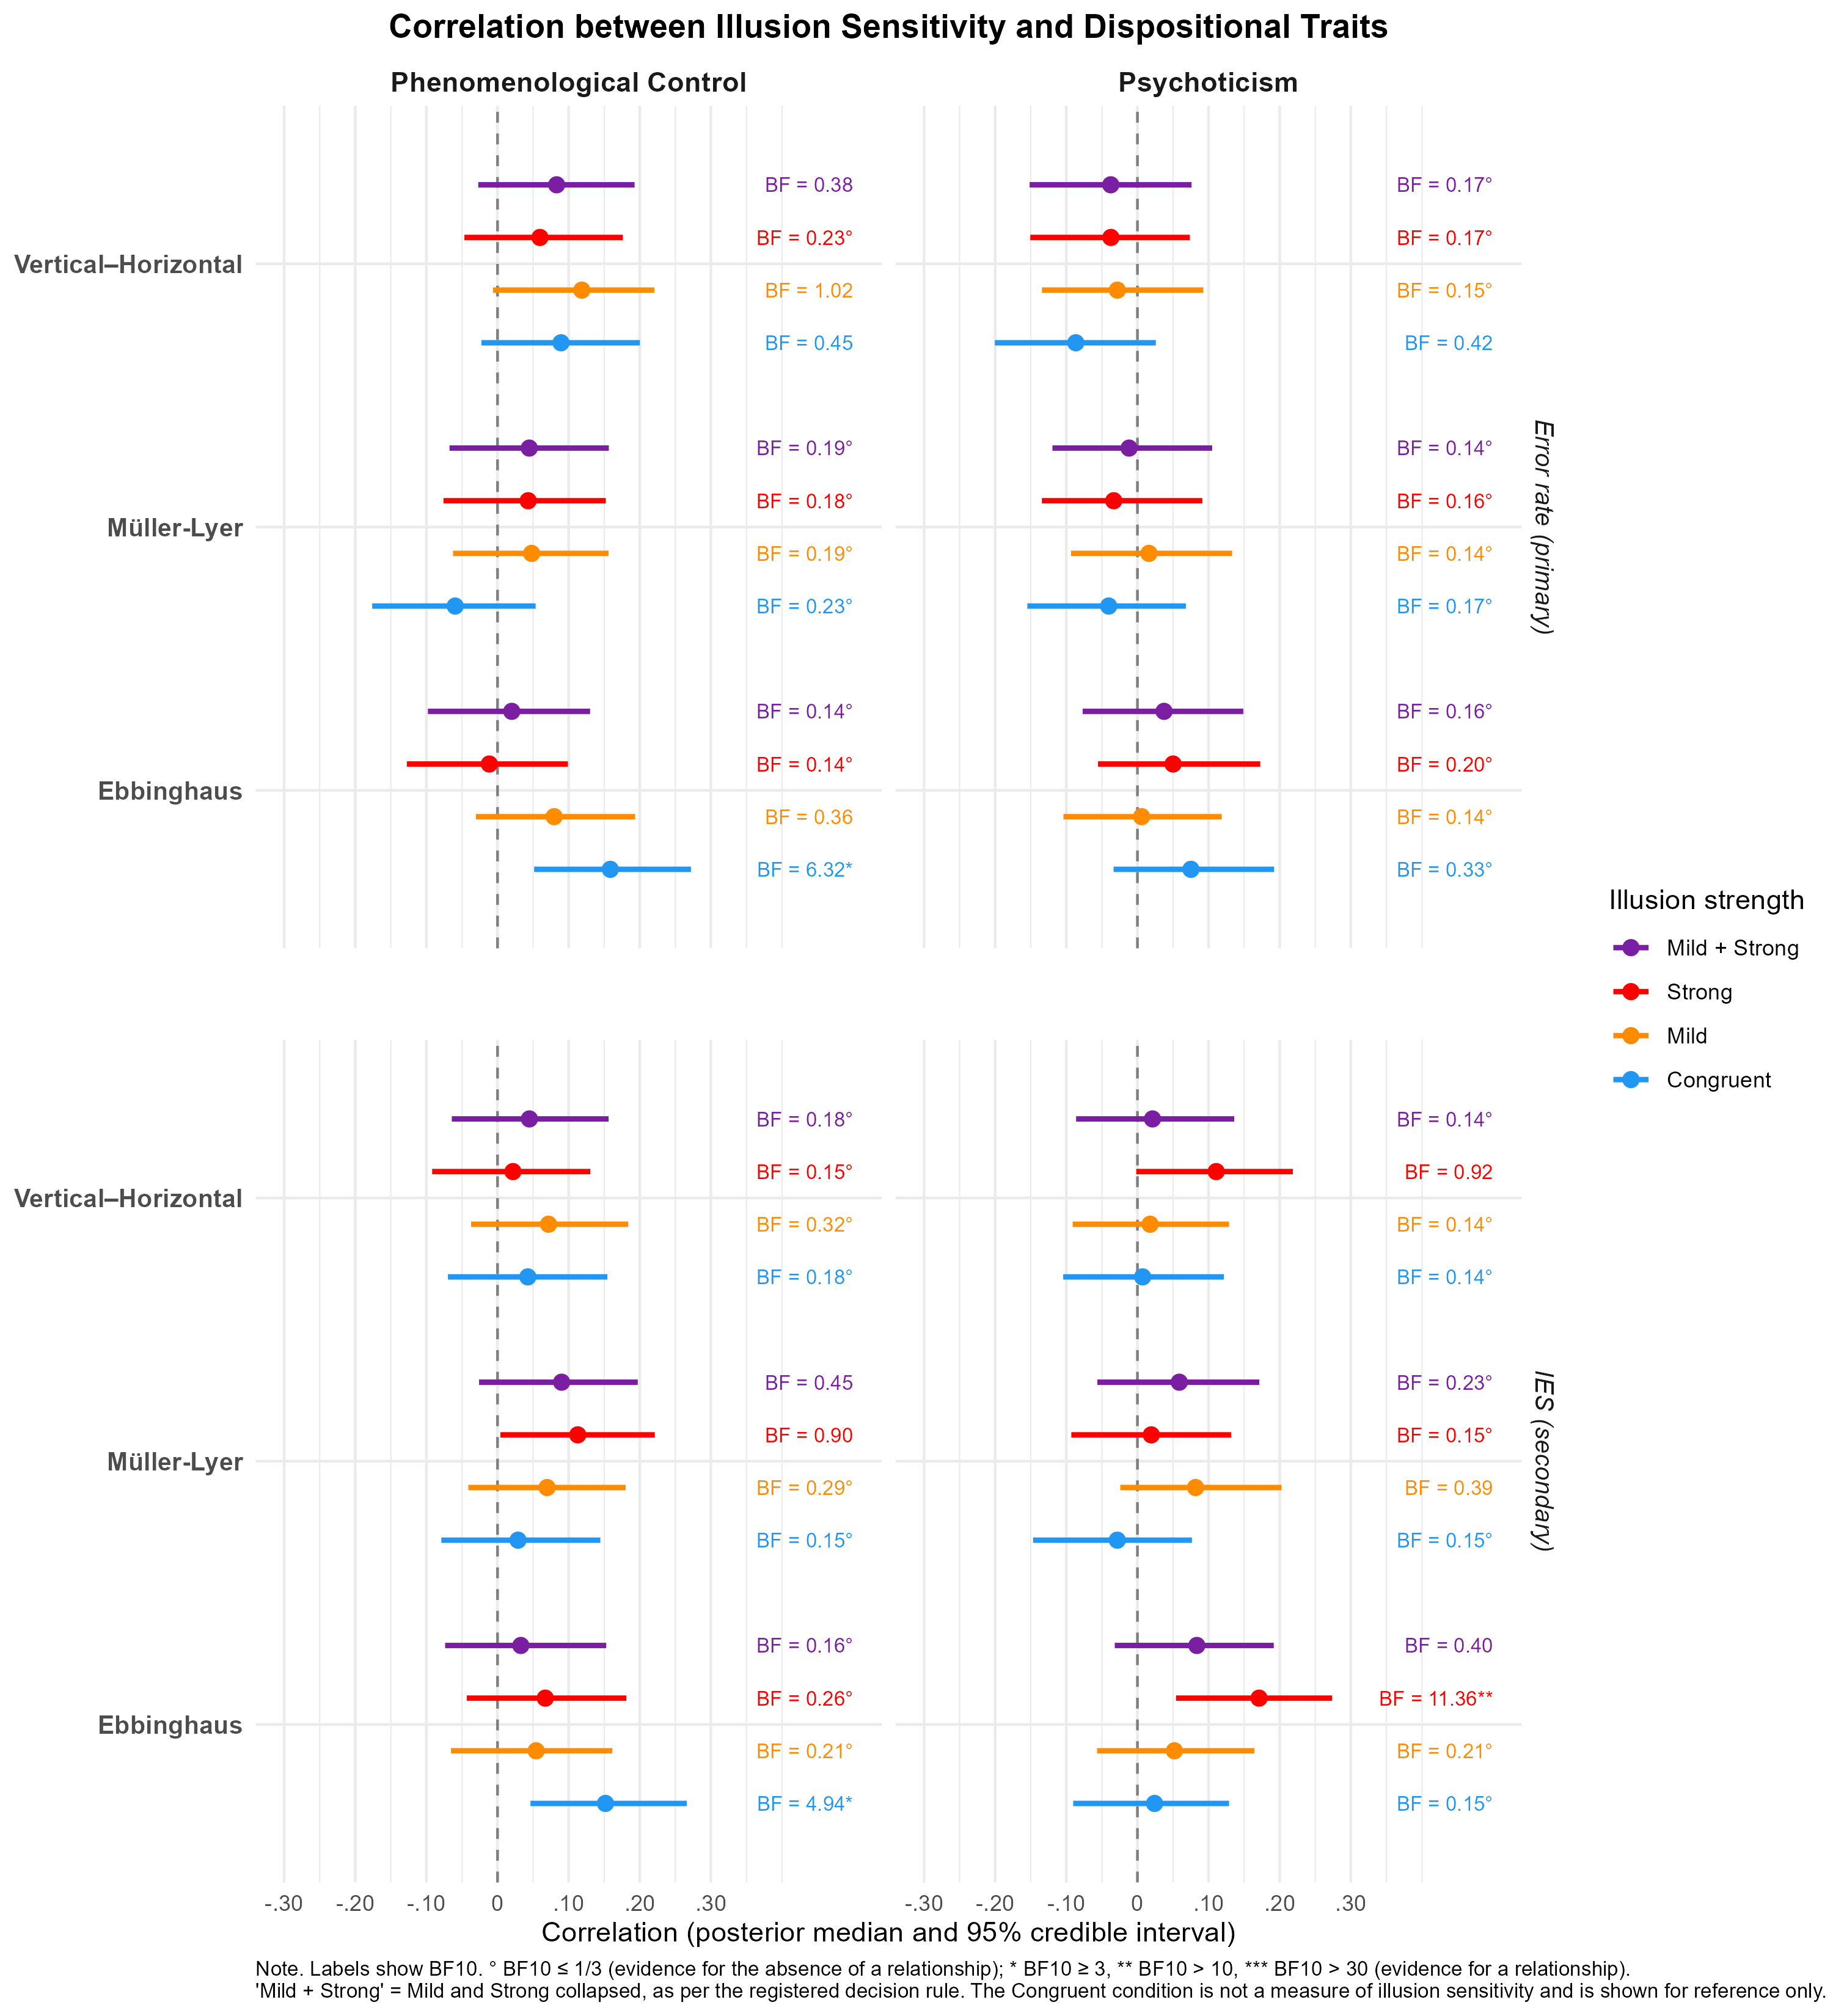
\includegraphics[width=1\linewidth,height=\textheight,keepaspectratio]{../../analysis/figures/fig_correlations_registered.png}

}

\end{figure}%

\subsubsection{Sensitivity Analyses}\label{sensitivity-analyses}

\textbf{The registered analyses were repeated in the unregistered
analysis described in Deviations From Registration, which addressed the
issues identified during analysis: the space bar check was not applied,
and extreme trials and participants with extreme congruent error rates
were excluded (N = 458 per illusion).} \textbf{The registered decision
rule for collapsing Mild and Strong was applied separately in this
sample, leading to the same decisions except for the IES of the
Müller-Lyer illusion, which was analysed separately (\emph{r} = .43;
Table S2).} \textbf{The effect of each deviation was also evaluated
separately (Table S1).} \textbf{Restricting the registered analysis to
native English speakers (N = 252), as specified in the Stage 1 protocol,
also led to the same conclusions for the primary outcome, with evidence
for the null for all three illusions (Vertical-Horizontal:
\(BF_{10} = 0.25\)).} \textbf{Restricting the registered analysis to
native English speakers (N = 252), as specified in the Stage 1 protocol,
also led to the same conclusions for the primary outcome.} \textbf{None
of these changes altered the conclusions for the primary outcome: in the
unregistered analysis, PCS was unrelated to error rates for the
Müller-Lyer (\(BF_{10} = 0.11\)) and Ebbinghaus illusions
(\(BF_{10} = 0.11\)), the evidence for the Vertical-Horizontal illusion
remained inconclusive (\(BF_{10} = 0.42\)), and all psychoticism--error
rate correlations supported the null (\(BF_{10} = 0.11\)--\(0.20\)).}
\textbf{The classification of a few tests of the secondary outcome (IES)
lying close to the evidential thresholds varied between versions, but
none supported a relationship in the unregistered analysis.}

\subsubsection{Exploratory Analyses}\label{exploratory-analyses}

To ensure the robustness of these findings to various analysis
decisions, we additionally computed the correlations with variant scores
of the illusion game, namely with \textbf{Mild and Strong analysed
separately for all scores, and with outcomes computed separately for
each difficulty level (i.e., Easy and Hard).} \textbf{With Mild and
Strong analysed separately, 9 of the 12 PCS correlations supported the
null and 3 were inconclusive; across the 36 difficulty-specific PCS
correlations, 29 supported the null and 7 were inconclusive.} \textbf{No
PCS correlation supported a relationship.} \textbf{For psychoticism, one
correlation supported a relationship in both variants: IES for the
Ebbinghaus illusion in the Strong condition (Mild and Strong separate:
\emph{r} = .17, \(BF_{10} = 11.4\); Easy trials: \emph{r} = .17,
\(BF_{10} = 11.2\)), which was positive, i.e., in the direction opposite
to the registered hypothesis.} \textbf{All other psychoticism
correlations supported the null or were inconclusive.} \textbf{Finally,
PCS correlated with the error rate (\(BF_{10} = 6.32\)) and IES
(\(BF_{10} = 4.94\)) in the congruent condition of the Ebbinghaus
illusion (Figure~\ref{fig-corr}); as the congruent condition does not
index illusion sensitivity, these correlations were not part of the
registered tests and should be interpreted with caution.}

\section{Discussion}\label{discussion}

This study aimed to replicate previous findings indicating (1) an
absence of a relationship between visual illusion sensitivity and
phenomenological control (\citeproc{ref-lush2022}{Lush et al., 2022}),
and (2) the existence of a \textbf{negative} relationship between
illusion sensitivity and psychoticism
(\citeproc{ref-makowski2023}{Makowski et al., 2023}). \textbf{For the
primary outcome (error rate), registered Bayesian correlation analyses
provided evidence against a relationship between phenomenological
control and sensitivity to two of the three illusions tested
(Müller-Lyer and Ebbinghaus), whereas the evidence for the third
(Vertical-Horizontal) was inconclusive, partly supporting the first
hypothesis.} \textbf{The data also favoured the absence of an
association between illusion sensitivity and psychoticism, contrary to
the second hypothesis.} \textbf{These conclusions were robust to the
data quality issues identified during analysis: an unregistered analysis
that addressed them, with a larger sample, did not change any conclusion
for the primary outcome.}

The present findings \textbf{partly replicate Lush et al.
(\citeproc{ref-lush2022}{2022}).} \textbf{For the primary outcome, we
obtained evidence against a relationship between trait phenomenological
control (PC) and sensitivity to the Müller-Lyer and Ebbinghaus
illusions, whereas the evidence for the Vertical-Horizontal illusion was
inconclusive.} Crucially, while previous research relied largely on
subjective metacognitive judgments, our use of the Illusion Game
paradigm extends this null finding to a direct, behavioral measure of
perceptual interference. This \textbf{pattern is consistent with} the
cognitive impenetrability of \textbf{these illusions under the present
task conditions.} Although both PC and illusion susceptibility can be
conceptualized as top-down processes, our results suggest they operate
at different levels of the cognitive hierarchy. The perceptual priors
assumed to drive illusion sensitivity might be organized in a modular
and encapsulated fashion. Consequently, even individuals with a high
capacity to alter their subjective experience in response to goals or
expectations (high PC) \textbf{do not appear to exert high-level},
goal-directed control over these low-level perceptual inferences. In
practice, this suggests that the trait capacity to manipulate one's
phenomenology is insufficient to override the behavioural interference
\textbf{of these illusions}. \textbf{The inconclusive result for the
Vertical-Horizontal illusion, however, indicates that this conclusion
cannot be extended to all three illusions tested.}

In contrast to our registered hypothesis, we found no evidence of an
association between visual illusion sensitivity and the psychoticism
facet of the PID-5; \textbf{for the primary outcome, the Bayes factors
favoured the absence of an association rather than being merely
uninformative.} This result was unexpected, given the literature linking
schizophrenia-spectrum traits and schizotypy to reduced susceptibility
to visual illusions, a phenomenon often attributed to the reduced
precision of perceptual priors within predictive coding frameworks.
\textbf{One possible contributor is the limited variability of
psychoticism in our general-population sample: scores were low on
average (\emph{M} = 0.48 on a 0--3 scale) and positively skewed, with
most participants scoring near the bottom of the scale (Figure S2).}
\textbf{Such a restricted range limits the ability to detect
associations.} However, this discrepancy may also be driven by how
individual differences were operationalized in the current study. For
instance, whereas Makowski et al. (\citeproc{ref-makowski2023}{2023})
measured sensitivity across an aggregate of 10 different visual
illusions, the current procedure was streamlined to include only three,
\textbf{and the relationship with psychoticism was analyzed for each
illusion individually.} We may therefore have lacked the statistical
breadth required to extract a robust, common ``illusion sensitivity''
factor. Conceptually, we could hypothesize that the task-performance on
any single illusion is driven by a combination of illusion-specific
factors (e.g., the particular perceptual properties and localized
prior-systems engaged by that specific visual configuration) and
illusion-general factors (an overarching, trait-level characteristic
tapped into during illusory perceptual interference). When analyzing
specific illusions in isolation, the illusion-specific factors might
overweigh the common component, potentially masking associations with
broad personality constructs. However, this assumption is challenged by
the fact that the internal consistency (i.e., the inter-correlation)
between the three illusions in our sample was remarkably low,
inconsistent at first glance with the notion of a common ``illusion
sensitivity'' factor. This lack of coherence might result from a
compounding of issues related to both the low number of illusions, as
well as the specific measurement indices utilized.

Indeed, it is important to underline that the above findings and
hypotheses are predicated on one critical assumption: that the outcome
measures used in the current study (error rate and IES) are valid and
sensitive indices to the individual differences in illusion sensitivity.
Previous studies that successfully detected relationships with
personality traits, such as Makowski et al.
(\citeproc{ref-makowski2023}{2023}), utilized indices derived from
participant-specific parameters extracted from group-level hierarchical
Bayesian General Additive Models (GAMs). In contrast, the current
pre-registered analysis intentionally relied on rather crude summary
measures. This critical methodological trade-off regarding how
perceptual interference is quantified was adopted as complex
computational models, while sensitive, carry significant drawbacks. For
instance, they are computationally challenging and complex, and the
resulting individual indices are not easily reproducible and replicable
(as the estimates are inherently dependent on a bespoke parent model
estimated from a specific dataset). Moreover, they are inherently
limited by the appropriateness of the parent model as an accurate
representation of the underlying data-generating process, which as noted
by Makowski et al. (\citeproc{ref-makowski2023}{2023}), is not yet
established. In particular, while the GAMs used are great models to
describe complex, potentially non-linear, patterns and relationships,
they did not account for the interaction between speed and accuracy,
which might be an important aspect of illusion-related perceptual
interference effects. But while our chosen summary metrics provided a
straightforward, reproducible index of performance, collapsing the
variance across task difficulty, illusion strength, and speed-accuracy
trade-offs might have stripped away the nuanced resolution required to
detect the subtle, low-level individual differences associated with
personality-level characteristics. \textbf{The sensitivity of the tests
was further limited by the sample size of the registered analysis:
applying the registered space bar check reduced the sample from 468 to
295 participants, and the inconclusive results (concentrated in the
Vertical-Horizontal illusion and the secondary outcome) may partly
reflect this reduced sensitivity rather than evidence for a
relationship.} \textbf{Notably, the unregistered analysis, with a larger
sample, led to the same conclusions for the primary outcome.}

Another important consideration for contextualizing these findings lies
in the specific cognitive demands of the Illusion Game and the
distinction between trait and state phenomenological control. In our
paradigm, participants were explicitly motivated to respond as quickly
and accurately as possible, effectively incentivizing them to actively
inhibit or ``resist'' the illusory interference. This voluntary,
goal-directed attempt to suppress a visual bias likely mobilizes
distinct cognitive mechanisms compared to contexts where individuals are
simply invited to passively experience or contemplate an illusion. In
such contemplative settings, individuals might even implicitly magnify
the illusory effect for aesthetic or psychological engagement.
Furthermore, the present study measured trait phenomenological control,
the baseline capacity for altering subjective experience, but did not
provide an explicit induction or suggestion to alter the perception of
the stimuli (i.e., state phenomenological control). \textbf{Moreover,
while the task instructions provided a clear goal (to respond accurately
despite the illusion), they did not provide any strategy for achieving
it, and motivation to overcome an illusion is distinct from knowing how
to do so.} \textbf{The present results therefore concern the
relationship between trait phenomenological control and illusion
susceptibility, and do not speak to whether state-dependent
interventions (e.g., a specific suggestion or strategy) could confer
behavioural control over these illusions.} \textbf{Future studies could
test whether explicitly providing potentially effective strategies, such
as those shown to reduce Stroop interference
(\citeproc{ref-palfi2022}{Palfi et al., 2022}), reduces susceptibility
to these illusions, and whether the present instructions are sufficient
to reduce interference in tasks in which cognitive penetration is known
to be possible.} Typical PC tasks assess the ability to generate or
facilitate a suggested experience (e.g., feeling a heavy arm), whereas
our task required the suppression of a bottom-up perceptual signal. It
remains an open question whether a strong, context-specific suggestion
(e.g., ``you will see the lines exactly as their physical length
dictates'') could mobilize state phenomenological control sufficiently
to penetrate these encapsulated perceptual priors. Consequently, our
results should \textbf{not} be over-generalized and are best framed
specifically as suggesting that high \emph{trait capacity} for
phenomenological control does not automatically confer an enhanced
ability to \emph{actively} inhibit \textbf{these} perceptual illusions
under strict, performance-driven task demands.

In summary, the present study \textbf{suggests that sensitivity to the
Müller-Lyer and Ebbinghaus illusions operates} to a large extent
independently of our trait-level capacity to alter subjective
phenomenology. \textbf{Importantly, three illusions are not a
representative sample of visual illusions, and their low
inter-correlation in the present data suggests that performance on each
of them is largely driven by illusion-specific mechanisms.} \textbf{Our
conclusions therefore apply to the illusions for which evidence for the
null was obtained, rather than to visual illusions in general.} However,
our findings also highlight a critical methodological bottleneck in the
study of perceptual individual differences. The lack of correlation
between illusion sensitivity and psychoticism, coupled with low
inter-illusion consistency, suggests that simple summary metrics derived
from a small subset of illusions are insufficient to capture broad
perceptual traits. Future research aiming to map low-level perceptual
priors onto higher-order personality or psychopathological constructs
must bridge the gap between reproducibility and modeling sensitivity.
This could involve utilizing computational frameworks that explicitly
model the speed-accuracy trade-off, such as Drift Diffusion Models
(DDMs), to disentangle true perceptual bias from response impulsivity.
Furthermore, developing standardized, multi-illusion batteries will be
essential for successfully isolating a common, trait-level ``illusion
sensitivity'' factor from the noise of illusion-specific variance. Until
such high-resolution, reliable metrics are established, the subtle links
between subclinical maladaptive traits and predictive coding parameters
might remain difficult to capture.

\section{Data Availability}\label{data-availability}

All the study materials, experiment, data, and analysis are available on
GitHub at
\textbf{https://github.com/RealityBending/IllusionGamePhenomenologicalControl}.

This study was pre-registered as a Registered Report
(https://osf.io/kvjnm) following Stage 1 in-principle acceptance on the
5/12/2025.

\section{Acknowledgments}\label{acknowledgments}

We would like to thank Oliver Collins for his help in the last mile of
this project, An Shu Te for her help in setting it up, Ryan Scott for
his help in implementing the phenomenological control scale, and Zoltan
Dienes for his input, feedback and guidance.

\section{Conflict of Interest
Disclosure}\label{conflict-of-interest-disclosure}

\textbf{The authors of this article declare that they have no financial
conflict of interest with the content of this article.}

\pagebreak

\section{References}\label{references}

\protect\phantomsection\label{refs}
\begin{CSLReferences}{1}{0}
\bibitem[\citeproctext]{ref-cohen2013statistical}
Cohen, J. (2013). \emph{Statistical power analysis for the behavioral
sciences}. routledge.

\bibitem[\citeproctext]{ref-costa2023}
Costa, A. L. L., Costa, D. L., Pessoa, V. F., Caixeta, F. V., \& Maior,
R. S. (2023). Systematic review of visual illusions in schizophrenia.
\emph{Schizophrenia Research}, \emph{252}, 13--22.
\url{https://doi.org/10.1016/j.schres.2022.12.030}

\bibitem[\citeproctext]{ref-cronbach1951coefficient}
Cronbach, L. J. (1951). Coefficient alpha and the internal structure of
tests. \emph{Psychometrika}, \emph{16}(3), 297--334.

\bibitem[\citeproctext]{ref-de2015jspsych}
De Leeuw, J. R. (2015). jsPsych: A JavaScript library for creating
behavioral experiments in a web browser. \emph{Behavior Research
Methods}, \emph{47}, 1--12.

\bibitem[\citeproctext]{ref-deleeuw2023}
De Leeuw, J. R. (2023). DataPipe: Born-open data collection for online
experiments. \emph{Behavior Research Methods}, \emph{56}(3), 2499--2506.
\url{https://doi.org/10.3758/s13428-023-02161-x}

\bibitem[\citeproctext]{ref-dienes2022}
Dienes, Z., Lush, P., Palfi, B., Roseboom, W., Scott, R., Parris, B.,
Seth, A., \& Lovell, M. (2022). Phenomenological control as cold
control. \emph{Psychology of Consciousness: Theory, Research, and
Practice}, \emph{9}(2), 101--116.
\url{https://doi.org/10.1037/cns0000230}

\bibitem[\citeproctext]{ref-friston2010}
Friston, K. (2010). The free-energy principle: A unified brain theory?
\emph{Nature Reviews Neuroscience}, \emph{11}(2), 127--138.
\url{https://doi.org/10.1038/nrn2787}

\bibitem[\citeproctext]{ref-gershman2012}
Gershman, S. J., Vul, E., \& Tenenbaum, J. B. (2012). Multistability and
perceptual inference. \emph{Neural Computation}, \emph{24}(1), 1--24.
\url{https://doi.org/10.1162/neco_a_00226}

\bibitem[\citeproctext]{ref-gori2016}
Gori, S., Molteni, M., \& Facoetti, A. (2016). Visual illusions: An
interesting tool to investigate developmental dyslexia and autism
spectrum disorder. \emph{Frontiers in Human Neuroscience}, \emph{10}.
\url{https://doi.org/10.3389/fnhum.2016.00175}

\bibitem[\citeproctext]{ref-krueger2011}
Krueger, R. F., Eaton, N. R., Derringer, J., Markon, K. E., Watson, D.,
\& Skodol, A. E. (2011). Personality
in{\emph{DSM{\textendash}5:}}helping delineate personality disorder
content and framing the metastructure. \emph{Journal of Personality
Assessment}, \emph{93}(4), 325--331.
\url{https://doi.org/10.1080/00223891.2011.577478}

\bibitem[\citeproctext]{ref-parameters}
Lüdecke, D., Ben-Shachar, M. S., Patil, I., \& Makowski, D. (2020).
\emph{Extracting, computing and exploring the parameters of statistical
models using {\textbraceleft}r{\textbraceright}.} \emph{5}, 2445.
\url{https://doi.org/10.21105/joss.02445}

\bibitem[\citeproctext]{ref-easystats}
Lüdecke, D., Ben-Shachar, M. S., Patil, I., Wiernik, B. M., Bacher, E.,
Thériault, R., \& Makowski, D. (2022). \emph{Easystats: Framework for
easy statistical modeling, visualization, and reporting}.
\url{https://easystats.github.io/easystats/}

\bibitem[\citeproctext]{ref-lush2018}
Lush, P., Moga, G., McLatchie, N., \& Dienes, Z. (2018). The
sussex-waterloo scale of hypnotizability (SWASH): Measuring capacity for
altering conscious experience. \emph{Neuroscience of Consciousness},
\emph{2018}(1). \url{https://doi.org/10.1093/nc/niy006}

\bibitem[\citeproctext]{ref-lush2021}
Lush, P., Scott, R. B., Seth, A. K., \& Dienes, Z. (2021). The
phenomenological control scale: Measuring the capacity for creating
illusory nonvolition, hallucination and delusion. \emph{Collabra:
Psychology}, \emph{7}(1). \url{https://doi.org/10.1525/collabra.29542}

\bibitem[\citeproctext]{ref-lush2022}
Lush, P., Seth, A., Dienes, Z., \& Scott, R. B. (2022). \emph{Trait
phenomenological control in top-down and bottom-up effects: ASMR,
visually evoked auditory response and the müller-lyer illusion}.
\url{http://dx.doi.org/10.31234/osf.io/hw4y9}

\bibitem[\citeproctext]{ref-bayestestR}
Makowski, D., Ben-Shachar, M. S., \& Lüdecke, D. (2019).
\emph{bayestestR: Describing effects and their uncertainty, existence
and significance within the bayesian framework.} \emph{4}, 1541.
\url{https://doi.org/10.21105/joss.01541}

\bibitem[\citeproctext]{ref-makowski2021}
Makowski, D., Lau, Z. J., Pham, T., Paul Boyce, W., \& Annabel Chen, S.
H. (2021). A parametric framework to generate visual illusions using
python. \emph{Perception}, \emph{50}(11), 950--965.
\url{https://doi.org/10.1177/03010066211057347}

\bibitem[\citeproctext]{ref-makowski2023}
Makowski, D., Te, A. S., Kirk, S., Liang, N. Z., \& Chen, S. H. A.
(2023). A novel visual illusion paradigm provides evidence for a general
factor of illusion sensitivity and personality correlates.
\emph{Scientific Reports}, \emph{13}(1).
\url{https://doi.org/10.1038/s41598-023-33148-5}

\bibitem[\citeproctext]{ref-correlation}
Makowski, D., Wiernik, B. M., Patil, I., Lüdecke, D., \& Ben-Shachar, M.
S. (2022).
\emph{{\textbraceleft}{\textbraceleft}Correlation{\textbraceright}{\textbraceright}:
Methods for correlation analysis}.
\url{https://CRAN.R-project.org/package=correlation}

\bibitem[\citeproctext]{ref-mitchell2010}
Mitchell, P., Mottron, L., Soulières, I., \& Ropar, D. (2010).
Susceptibility to the shepard illusion in participants with autism:
Reduced top{-}down influences within perception? \emph{Autism Research},
\emph{3}(3), 113--119. \url{https://doi.org/10.1002/aur.130}

\bibitem[\citeproctext]{ref-morey2018baysefactor}
Morey, R. D., \& Rouder, J. N. (2018). \emph{BayseFactor: Computation of
bayes factors for common designs}.

\bibitem[\citeproctext]{ref-BayesFactor}
Morey, R. D., \& Rouder, J. N. (2024). \emph{BayesFactor: Computation of
bayes factors for common designs}.
\url{https://CRAN.R-project.org/package=BayesFactor}

\bibitem[\citeproctext]{ref-notredame2014}
Notredame, C.-E., Pins, D., Deneve, S., \& Jardri, R. (2014). What
visual illusions teach us about schizophrenia. \emph{Frontiers in
Integrative Neuroscience}, \emph{8}.
\url{https://doi.org/10.3389/fnint.2014.00063}

\bibitem[\citeproctext]{ref-nour2015perception}
Nour, M. M., \& Nour, J. M. (2015). Perception, illusions and bayesian
inference. \emph{Psychopathology}, \emph{48}(4), 217--221.

\bibitem[\citeproctext]{ref-palfi2022}
Palfi, B., Parris, B. A., Collins, A. F., \& Dienes, Z. (2022).
Strategies that reduce stroop interference. \emph{Royal Society Open
Science}, \emph{9}(3), 202136. \url{https://doi.org/10.1098/rsos.202136}

\bibitem[\citeproctext]{ref-palmer2017}
Palmer, C. J., Lawson, R. P., \& Hohwy, J. (2017). Bayesian approaches
to autism: Towards volatility, action, and behavior. \emph{Psychological
Bulletin}, \emph{143}(5), 521--542.
\url{https://doi.org/10.1037/bul0000097}

\bibitem[\citeproctext]{ref-datawizard}
Patil, I., Makowski, D., Ben-Shachar, M. S., Wiernik, B. M., Bacher, E.,
\& Lüdecke, D. (2022).
\emph{{\textbraceleft}Datawizard{\textbraceright}: An
{\textbraceleft}r{\textbraceright} package for easy data preparation and
statistical transformations}. \emph{7}, 4684.
\url{https://doi.org/10.21105/joss.04684}

\bibitem[\citeproctext]{ref-shoshina2014}
Shoshina, I. I., \& Shelepin, Yu. E. (2014). Effectiveness of
discrimination of the sizes of line segments by humans with different
cognitive style parameters. \emph{Neuroscience and Behavioral
Physiology}, \emph{44}(7), 748--753.
\url{https://doi.org/10.1007/s11055-014-9978-2}

\bibitem[\citeproctext]{ref-sibley2011mini}
{Sibley, C. G., Luyten, N., Purnomo, M., Mobberley, A., Wootton, L. W.,
Hammond, M. D., Sengupta, N., Perry, R., West-Newman, T., Wilson, M. S.,
et al.} (2011). The mini-IPIP6: Validation and extension of a short
measure of the big-six factors of personality in new zealand. \emph{New
Zealand Journal of Psychology}, \emph{40}(3).

\bibitem[\citeproctext]{ref-sundareswara2008}
Sundareswara, R., \& Schrater, P. R. (2008). Perceptual multistability
predicted by search model for bayesian decisions. \emph{Journal of
Vision}, \emph{8}(5), 12. \url{https://doi.org/10.1167/8.5.12}

\bibitem[\citeproctext]{ref-theriault2024}
Thériault, R., Ben-Shachar, M. S., Patil, I., Lüdecke, D., Wiernik, B.
M., \& Makowski, D. (2024). Check your outliers! An introduction to
identifying statistical outliers in r with easystats. \emph{Behavior
Research Methods}. \url{https://doi.org/10.3758/s13428-024-02356-w}

\bibitem[\citeproctext]{ref-todorovic2020}
Todorović, D. (2020). What are visual illusions? \emph{Perception},
\emph{49}(11), 1128--1199.
\url{https://doi.org/10.1177/0301006620962279}

\bibitem[\citeproctext]{ref-townsend2014methods}
Townsend, J. T., \& Ashby, F. G. (2014). Methods of modeling capacity in
simple processing systems. In \emph{Cognitive theory} (pp. 199--239).
Psychology Press.

\bibitem[\citeproctext]{ref-tidyverse}
Wickham, H., Averick, M., Bryan, J., Chang, W., McGowan, L. D.,
François, R., Grolemund, G., Hayes, A., Henry, L., Hester, J., Kuhn, M.,
Pedersen, T. L., Miller, E., Bache, S. M., Müller, K., Ooms, J.,
Robinson, D., Seidel, D. P., Spinu, V., \ldots{} Yutani, H. (2019).
\emph{Welcome to the {\textbraceleft}tidyverse{\textbraceright}}.
\emph{4}, 1686. \url{https://doi.org/10.21105/joss.01686}

\end{CSLReferences}

\pagebreak

\appendix

\section{Supplementary Materials}\label{apx-supplementary-materials}

\textbf{Table S1}

\textbf{\emph{Number of registered tests supporting the null /
inconclusive / supporting a relationship under each version of the
analysis}}

\global\setlength{\Oldarrayrulewidth}{\arrayrulewidth}

\global\setlength{\Oldtabcolsep}{\tabcolsep}

\setlength{\tabcolsep}{2pt}

\renewcommand*{\arraystretch}{1.5}



\providecommand{\ascline}[3]{\noalign{\global\arrayrulewidth #1}\arrayrulecolor[HTML]{#2}\cline{#3}}

\begin{longtable*}[c]{cccccc}



\ascline{1.5pt}{666666}{1-6}

\multicolumn{1}{>{}l}{\advance\leftskip by 5.0pt\relax \advance\rightskip by 5.0pt\relax \textcolor[HTML]{000000}{\fontsize{9}{9}\selectfont{{\fontspec{Arial} Analysis}}}} & \multicolumn{1}{>{}l}{\advance\leftskip by 5.0pt\relax \advance\rightskip by 5.0pt\relax \textcolor[HTML]{000000}{\fontsize{9}{9}\selectfont{{\fontspec{Arial} N}}}} & \multicolumn{1}{>{}l}{\advance\leftskip by 5.0pt\relax \advance\rightskip by 5.0pt\relax \textcolor[HTML]{000000}{\fontsize{9}{9}\selectfont{{\fontspec{Arial} PCS\ ×\ Error\ rate}}}} & \multicolumn{1}{>{}l}{\advance\leftskip by 5.0pt\relax \advance\rightskip by 5.0pt\relax \textcolor[HTML]{000000}{\fontsize{9}{9}\selectfont{{\fontspec{Arial} PCS\ ×\ IES}}}} & \multicolumn{1}{>{}l}{\advance\leftskip by 5.0pt\relax \advance\rightskip by 5.0pt\relax \textcolor[HTML]{000000}{\fontsize{9}{9}\selectfont{{\fontspec{Arial} Psychoticism\ ×\ Error\ rate}}}} & \multicolumn{1}{>{}l}{\advance\leftskip by 5.0pt\relax \advance\rightskip by 5.0pt\relax \textcolor[HTML]{000000}{\fontsize{9}{9}\selectfont{{\fontspec{Arial} Psychoticism\ ×\ IES}}}} \\

\ascline{1.5pt}{666666}{1-6}\endfirsthead 

\ascline{1.5pt}{666666}{1-6}

\multicolumn{1}{>{}l}{\advance\leftskip by 5.0pt\relax \advance\rightskip by 5.0pt\relax \textcolor[HTML]{000000}{\fontsize{9}{9}\selectfont{{\fontspec{Arial} Analysis}}}} & \multicolumn{1}{>{}l}{\advance\leftskip by 5.0pt\relax \advance\rightskip by 5.0pt\relax \textcolor[HTML]{000000}{\fontsize{9}{9}\selectfont{{\fontspec{Arial} N}}}} & \multicolumn{1}{>{}l}{\advance\leftskip by 5.0pt\relax \advance\rightskip by 5.0pt\relax \textcolor[HTML]{000000}{\fontsize{9}{9}\selectfont{{\fontspec{Arial} PCS\ ×\ Error\ rate}}}} & \multicolumn{1}{>{}l}{\advance\leftskip by 5.0pt\relax \advance\rightskip by 5.0pt\relax \textcolor[HTML]{000000}{\fontsize{9}{9}\selectfont{{\fontspec{Arial} PCS\ ×\ IES}}}} & \multicolumn{1}{>{}l}{\advance\leftskip by 5.0pt\relax \advance\rightskip by 5.0pt\relax \textcolor[HTML]{000000}{\fontsize{9}{9}\selectfont{{\fontspec{Arial} Psychoticism\ ×\ Error\ rate}}}} & \multicolumn{1}{>{}l}{\advance\leftskip by 5.0pt\relax \advance\rightskip by 5.0pt\relax \textcolor[HTML]{000000}{\fontsize{9}{9}\selectfont{{\fontspec{Arial} Psychoticism\ ×\ IES}}}} \\

\ascline{1.5pt}{666666}{1-6}\endhead



\multicolumn{6}{>{}l}{\advance\leftskip by 5.0pt\relax \advance\rightskip by 5.0pt\relax \textcolor[HTML]{000000}{\fontsize{9}{9}\selectfont{{\fontspec{Arial} Note.\ Each\ cell\ gives\ the\ number\ of\ tests\ with\ BF₁₀\ ≤\ 1/3\ (null)\ /\ inconclusive\ /\ BF₁₀\ ≥\ 3\ (relationship).\ N\ is\ the\ number\ of\ participants\ analysed\ (per\ illusion\ where\ it\ varies).}}}} \\

\endlastfoot



\multicolumn{1}{>{}l}{\advance\leftskip by 5.0pt\relax \advance\rightskip by 5.0pt\relax \textcolor[HTML]{000000}{\fontsize{9}{9}\selectfont{{\fontspec{Arial} Registered\ analysis\ (main\ analysis)}}}} & \multicolumn{1}{>{}l}{\advance\leftskip by 5.0pt\relax \advance\rightskip by 5.0pt\relax \textcolor[HTML]{000000}{\fontsize{9}{9}\selectfont{{\fontspec{Arial} 295}}}} & \multicolumn{1}{>{}l}{\advance\leftskip by 5.0pt\relax \advance\rightskip by 5.0pt\relax \textcolor[HTML]{000000}{\fontsize{9}{9}\selectfont{{\fontspec{Arial} 2\ /\ 1\ /\ 0}}}} & \multicolumn{1}{>{}l}{\advance\leftskip by 5.0pt\relax \advance\rightskip by 5.0pt\relax \textcolor[HTML]{000000}{\fontsize{9}{9}\selectfont{{\fontspec{Arial} 3\ /\ 1\ /\ 0}}}} & \multicolumn{1}{>{}l}{\advance\leftskip by 5.0pt\relax \advance\rightskip by 5.0pt\relax \textcolor[HTML]{000000}{\fontsize{9}{9}\selectfont{{\fontspec{Arial} 3\ /\ 0\ /\ 0}}}} & \multicolumn{1}{>{}l}{\advance\leftskip by 5.0pt\relax \advance\rightskip by 5.0pt\relax \textcolor[HTML]{000000}{\fontsize{9}{9}\selectfont{{\fontspec{Arial} 2\ /\ 2\ /\ 0}}}} \\





\multicolumn{1}{>{}l}{\advance\leftskip by 5.0pt\relax \advance\rightskip by 5.0pt\relax \textcolor[HTML]{000000}{\fontsize{9}{9}\selectfont{{\fontspec{Arial} Unregistered\ analysis\ (all\ deviations)}}}} & \multicolumn{1}{>{}l}{\advance\leftskip by 5.0pt\relax \advance\rightskip by 5.0pt\relax \textcolor[HTML]{000000}{\fontsize{9}{9}\selectfont{{\fontspec{Arial} 458}}}} & \multicolumn{1}{>{}l}{\advance\leftskip by 5.0pt\relax \advance\rightskip by 5.0pt\relax \textcolor[HTML]{000000}{\fontsize{9}{9}\selectfont{{\fontspec{Arial} 2\ /\ 1\ /\ 0}}}} & \multicolumn{1}{>{}l}{\advance\leftskip by 5.0pt\relax \advance\rightskip by 5.0pt\relax \textcolor[HTML]{000000}{\fontsize{9}{9}\selectfont{{\fontspec{Arial} 4\ /\ 1\ /\ 0}}}} & \multicolumn{1}{>{}l}{\advance\leftskip by 5.0pt\relax \advance\rightskip by 5.0pt\relax \textcolor[HTML]{000000}{\fontsize{9}{9}\selectfont{{\fontspec{Arial} 3\ /\ 0\ /\ 0}}}} & \multicolumn{1}{>{}l}{\advance\leftskip by 5.0pt\relax \advance\rightskip by 5.0pt\relax \textcolor[HTML]{000000}{\fontsize{9}{9}\selectfont{{\fontspec{Arial} 3\ /\ 2\ /\ 0}}}} \\





\multicolumn{1}{>{}l}{\advance\leftskip by 5.0pt\relax \advance\rightskip by 5.0pt\relax \textcolor[HTML]{000000}{\fontsize{9}{9}\selectfont{{\fontspec{Arial} Registered\ analysis,\ native\ English\ speakers\ only}}}} & \multicolumn{1}{>{}l}{\advance\leftskip by 5.0pt\relax \advance\rightskip by 5.0pt\relax \textcolor[HTML]{000000}{\fontsize{9}{9}\selectfont{{\fontspec{Arial} 252}}}} & \multicolumn{1}{>{}l}{\advance\leftskip by 5.0pt\relax \advance\rightskip by 5.0pt\relax \textcolor[HTML]{000000}{\fontsize{9}{9}\selectfont{{\fontspec{Arial} 3\ /\ 0\ /\ 0}}}} & \multicolumn{1}{>{}l}{\advance\leftskip by 5.0pt\relax \advance\rightskip by 5.0pt\relax \textcolor[HTML]{000000}{\fontsize{9}{9}\selectfont{{\fontspec{Arial} 3\ /\ 1\ /\ 0}}}} & \multicolumn{1}{>{}l}{\advance\leftskip by 5.0pt\relax \advance\rightskip by 5.0pt\relax \textcolor[HTML]{000000}{\fontsize{9}{9}\selectfont{{\fontspec{Arial} 3\ /\ 0\ /\ 0}}}} & \multicolumn{1}{>{}l}{\advance\leftskip by 5.0pt\relax \advance\rightskip by 5.0pt\relax \textcolor[HTML]{000000}{\fontsize{9}{9}\selectfont{{\fontspec{Arial} 2\ /\ 2\ /\ 0}}}} \\





\multicolumn{1}{>{}l}{\advance\leftskip by 5.0pt\relax \advance\rightskip by 5.0pt\relax \textcolor[HTML]{000000}{\fontsize{9}{9}\selectfont{{\fontspec{Arial} Registered\ criteria\ without\ the\ space\ bar\ check\ only}}}} & \multicolumn{1}{>{}l}{\advance\leftskip by 5.0pt\relax \advance\rightskip by 5.0pt\relax \textcolor[HTML]{000000}{\fontsize{9}{9}\selectfont{{\fontspec{Arial} 468}}}} & \multicolumn{1}{>{}l}{\advance\leftskip by 5.0pt\relax \advance\rightskip by 5.0pt\relax \textcolor[HTML]{000000}{\fontsize{9}{9}\selectfont{{\fontspec{Arial} 2\ /\ 1\ /\ 0}}}} & \multicolumn{1}{>{}l}{\advance\leftskip by 5.0pt\relax \advance\rightskip by 5.0pt\relax \textcolor[HTML]{000000}{\fontsize{9}{9}\selectfont{{\fontspec{Arial} 3\ /\ 2\ /\ 0}}}} & \multicolumn{1}{>{}l}{\advance\leftskip by 5.0pt\relax \advance\rightskip by 5.0pt\relax \textcolor[HTML]{000000}{\fontsize{9}{9}\selectfont{{\fontspec{Arial} 3\ /\ 0\ /\ 0}}}} & \multicolumn{1}{>{}l}{\advance\leftskip by 5.0pt\relax \advance\rightskip by 5.0pt\relax \textcolor[HTML]{000000}{\fontsize{9}{9}\selectfont{{\fontspec{Arial} 1\ /\ 3\ /\ 1}}}} \\





\multicolumn{1}{>{}l}{\advance\leftskip by 5.0pt\relax \advance\rightskip by 5.0pt\relax \textcolor[HTML]{000000}{\fontsize{9}{9}\selectfont{{\fontspec{Arial} Unregistered\ analysis\ without\ the\ trial\ exclusions}}}} & \multicolumn{1}{>{}l}{\advance\leftskip by 5.0pt\relax \advance\rightskip by 5.0pt\relax \textcolor[HTML]{000000}{\fontsize{9}{9}\selectfont{{\fontspec{Arial} 460–463}}}} & \multicolumn{1}{>{}l}{\advance\leftskip by 5.0pt\relax \advance\rightskip by 5.0pt\relax \textcolor[HTML]{000000}{\fontsize{9}{9}\selectfont{{\fontspec{Arial} 2\ /\ 1\ /\ 0}}}} & \multicolumn{1}{>{}l}{\advance\leftskip by 5.0pt\relax \advance\rightskip by 5.0pt\relax \textcolor[HTML]{000000}{\fontsize{9}{9}\selectfont{{\fontspec{Arial} 4\ /\ 1\ /\ 0}}}} & \multicolumn{1}{>{}l}{\advance\leftskip by 5.0pt\relax \advance\rightskip by 5.0pt\relax \textcolor[HTML]{000000}{\fontsize{9}{9}\selectfont{{\fontspec{Arial} 3\ /\ 0\ /\ 0}}}} & \multicolumn{1}{>{}l}{\advance\leftskip by 5.0pt\relax \advance\rightskip by 5.0pt\relax \textcolor[HTML]{000000}{\fontsize{9}{9}\selectfont{{\fontspec{Arial} 1\ /\ 4\ /\ 0}}}} \\





\multicolumn{1}{>{}l}{\advance\leftskip by 5.0pt\relax \advance\rightskip by 5.0pt\relax \textcolor[HTML]{000000}{\fontsize{9}{9}\selectfont{{\fontspec{Arial} Unregistered\ analysis\ without\ the\ participant\ exclusions\ (HDI)}}}} & \multicolumn{1}{>{}l}{\advance\leftskip by 5.0pt\relax \advance\rightskip by 5.0pt\relax \textcolor[HTML]{000000}{\fontsize{9}{9}\selectfont{{\fontspec{Arial} 468}}}} & \multicolumn{1}{>{}l}{\advance\leftskip by 5.0pt\relax \advance\rightskip by 5.0pt\relax \textcolor[HTML]{000000}{\fontsize{9}{9}\selectfont{{\fontspec{Arial} 2\ /\ 1\ /\ 0}}}} & \multicolumn{1}{>{}l}{\advance\leftskip by 5.0pt\relax \advance\rightskip by 5.0pt\relax \textcolor[HTML]{000000}{\fontsize{9}{9}\selectfont{{\fontspec{Arial} 4\ /\ 1\ /\ 0}}}} & \multicolumn{1}{>{}l}{\advance\leftskip by 5.0pt\relax \advance\rightskip by 5.0pt\relax \textcolor[HTML]{000000}{\fontsize{9}{9}\selectfont{{\fontspec{Arial} 3\ /\ 0\ /\ 0}}}} & \multicolumn{1}{>{}l}{\advance\leftskip by 5.0pt\relax \advance\rightskip by 5.0pt\relax \textcolor[HTML]{000000}{\fontsize{9}{9}\selectfont{{\fontspec{Arial} 3\ /\ 2\ /\ 0}}}} \\





\multicolumn{1}{>{}l}{\advance\leftskip by 5.0pt\relax \advance\rightskip by 5.0pt\relax \textcolor[HTML]{000000}{\fontsize{9}{9}\selectfont{{\fontspec{Arial} Registered\ analysis,\ Mild\ and\ Strong\ not\ collapsed\ (exploratory)}}}} & \multicolumn{1}{>{}l}{\advance\leftskip by 5.0pt\relax \advance\rightskip by 5.0pt\relax \textcolor[HTML]{000000}{\fontsize{9}{9}\selectfont{{\fontspec{Arial} 295}}}} & \multicolumn{1}{>{}l}{\advance\leftskip by 5.0pt\relax \advance\rightskip by 5.0pt\relax \textcolor[HTML]{000000}{\fontsize{9}{9}\selectfont{{\fontspec{Arial} 4\ /\ 2\ /\ 0}}}} & \multicolumn{1}{>{}l}{\advance\leftskip by 5.0pt\relax \advance\rightskip by 5.0pt\relax \textcolor[HTML]{000000}{\fontsize{9}{9}\selectfont{{\fontspec{Arial} 5\ /\ 1\ /\ 0}}}} & \multicolumn{1}{>{}l}{\advance\leftskip by 5.0pt\relax \advance\rightskip by 5.0pt\relax \textcolor[HTML]{000000}{\fontsize{9}{9}\selectfont{{\fontspec{Arial} 6\ /\ 0\ /\ 0}}}} & \multicolumn{1}{>{}l}{\advance\leftskip by 5.0pt\relax \advance\rightskip by 5.0pt\relax \textcolor[HTML]{000000}{\fontsize{9}{9}\selectfont{{\fontspec{Arial} 3\ /\ 2\ /\ 1}}}} \\

\ascline{1.5pt}{666666}{1-6}



\end{longtable*}



\arrayrulecolor[HTML]{000000}

\global\setlength{\arrayrulewidth}{\Oldarrayrulewidth}

\global\setlength{\tabcolsep}{\Oldtabcolsep}

\renewcommand*{\arraystretch}{1}

\textbf{Table S2}

\textbf{\emph{Correlations between the Mild and Strong conditions used
for the registered decision rule (collapsed if r \textgreater{} .50)}}

\global\setlength{\Oldarrayrulewidth}{\arrayrulewidth}

\global\setlength{\Oldtabcolsep}{\tabcolsep}

\setlength{\tabcolsep}{2pt}

\renewcommand*{\arraystretch}{1.5}



\providecommand{\ascline}[3]{\noalign{\global\arrayrulewidth #1}\arrayrulecolor[HTML]{#2}\cline{#3}}

\begin{longtable*}[c]{ccccc}



\ascline{1.5pt}{666666}{1-5}

\multicolumn{1}{>{}l}{\advance\leftskip by 5.0pt\relax \advance\rightskip by 5.0pt\relax \textcolor[HTML]{000000}{\fontsize{9}{9}\selectfont{{\fontspec{Arial} Analysis}}}} & \multicolumn{1}{>{}l}{\advance\leftskip by 5.0pt\relax \advance\rightskip by 5.0pt\relax \textcolor[HTML]{000000}{\fontsize{9}{9}\selectfont{{\fontspec{Arial} Outcome}}}} & \multicolumn{1}{>{}l}{\advance\leftskip by 5.0pt\relax \advance\rightskip by 5.0pt\relax \textcolor[HTML]{000000}{\fontsize{9}{9}\selectfont{{\fontspec{Arial} Illusion}}}} & \multicolumn{1}{>{}l}{\advance\leftskip by 5.0pt\relax \advance\rightskip by 5.0pt\relax \textcolor[HTML]{000000}{\fontsize{9}{9}\selectfont{{\fontspec{Arial} r}}}} & \multicolumn{1}{>{}l}{\advance\leftskip by 5.0pt\relax \advance\rightskip by 5.0pt\relax \textcolor[HTML]{000000}{\fontsize{9}{9}\selectfont{{\fontspec{Arial} Collapse}}}} \\

\ascline{1.5pt}{666666}{1-5}\endfirsthead 

\ascline{1.5pt}{666666}{1-5}

\multicolumn{1}{>{}l}{\advance\leftskip by 5.0pt\relax \advance\rightskip by 5.0pt\relax \textcolor[HTML]{000000}{\fontsize{9}{9}\selectfont{{\fontspec{Arial} Analysis}}}} & \multicolumn{1}{>{}l}{\advance\leftskip by 5.0pt\relax \advance\rightskip by 5.0pt\relax \textcolor[HTML]{000000}{\fontsize{9}{9}\selectfont{{\fontspec{Arial} Outcome}}}} & \multicolumn{1}{>{}l}{\advance\leftskip by 5.0pt\relax \advance\rightskip by 5.0pt\relax \textcolor[HTML]{000000}{\fontsize{9}{9}\selectfont{{\fontspec{Arial} Illusion}}}} & \multicolumn{1}{>{}l}{\advance\leftskip by 5.0pt\relax \advance\rightskip by 5.0pt\relax \textcolor[HTML]{000000}{\fontsize{9}{9}\selectfont{{\fontspec{Arial} r}}}} & \multicolumn{1}{>{}l}{\advance\leftskip by 5.0pt\relax \advance\rightskip by 5.0pt\relax \textcolor[HTML]{000000}{\fontsize{9}{9}\selectfont{{\fontspec{Arial} Collapse}}}} \\

\ascline{1.5pt}{666666}{1-5}\endhead



\multicolumn{1}{>{}l}{\advance\leftskip by 5.0pt\relax \advance\rightskip by 5.0pt\relax \textcolor[HTML]{000000}{\fontsize{9}{9}\selectfont{{\fontspec{Arial} Registered\ analysis}}}} & \multicolumn{1}{>{}l}{\advance\leftskip by 5.0pt\relax \advance\rightskip by 5.0pt\relax \textcolor[HTML]{000000}{\fontsize{9}{9}\selectfont{{\fontspec{Arial} Error\ rate}}}} & \multicolumn{1}{>{}l}{\advance\leftskip by 5.0pt\relax \advance\rightskip by 5.0pt\relax \textcolor[HTML]{000000}{\fontsize{9}{9}\selectfont{{\fontspec{Arial} Ebbinghaus}}}} & \multicolumn{1}{>{}l}{\advance\leftskip by 5.0pt\relax \advance\rightskip by 5.0pt\relax \textcolor[HTML]{000000}{\fontsize{9}{9}\selectfont{{\fontspec{Arial} 0.76}}}} & \multicolumn{1}{>{}l}{\advance\leftskip by 5.0pt\relax \advance\rightskip by 5.0pt\relax \textcolor[HTML]{000000}{\fontsize{9}{9}\selectfont{{\fontspec{Arial} Yes}}}} \\





\multicolumn{1}{>{}l}{\advance\leftskip by 5.0pt\relax \advance\rightskip by 5.0pt\relax \textcolor[HTML]{000000}{\fontsize{9}{9}\selectfont{{\fontspec{Arial} Registered\ analysis}}}} & \multicolumn{1}{>{}l}{\advance\leftskip by 5.0pt\relax \advance\rightskip by 5.0pt\relax \textcolor[HTML]{000000}{\fontsize{9}{9}\selectfont{{\fontspec{Arial} Error\ rate}}}} & \multicolumn{1}{>{}l}{\advance\leftskip by 5.0pt\relax \advance\rightskip by 5.0pt\relax \textcolor[HTML]{000000}{\fontsize{9}{9}\selectfont{{\fontspec{Arial} Müller-Lyer}}}} & \multicolumn{1}{>{}l}{\advance\leftskip by 5.0pt\relax \advance\rightskip by 5.0pt\relax \textcolor[HTML]{000000}{\fontsize{9}{9}\selectfont{{\fontspec{Arial} 0.67}}}} & \multicolumn{1}{>{}l}{\advance\leftskip by 5.0pt\relax \advance\rightskip by 5.0pt\relax \textcolor[HTML]{000000}{\fontsize{9}{9}\selectfont{{\fontspec{Arial} Yes}}}} \\





\multicolumn{1}{>{}l}{\advance\leftskip by 5.0pt\relax \advance\rightskip by 5.0pt\relax \textcolor[HTML]{000000}{\fontsize{9}{9}\selectfont{{\fontspec{Arial} Registered\ analysis}}}} & \multicolumn{1}{>{}l}{\advance\leftskip by 5.0pt\relax \advance\rightskip by 5.0pt\relax \textcolor[HTML]{000000}{\fontsize{9}{9}\selectfont{{\fontspec{Arial} Error\ rate}}}} & \multicolumn{1}{>{}l}{\advance\leftskip by 5.0pt\relax \advance\rightskip by 5.0pt\relax \textcolor[HTML]{000000}{\fontsize{9}{9}\selectfont{{\fontspec{Arial} Vertical-Horizontal}}}} & \multicolumn{1}{>{}l}{\advance\leftskip by 5.0pt\relax \advance\rightskip by 5.0pt\relax \textcolor[HTML]{000000}{\fontsize{9}{9}\selectfont{{\fontspec{Arial} 0.72}}}} & \multicolumn{1}{>{}l}{\advance\leftskip by 5.0pt\relax \advance\rightskip by 5.0pt\relax \textcolor[HTML]{000000}{\fontsize{9}{9}\selectfont{{\fontspec{Arial} Yes}}}} \\





\multicolumn{1}{>{}l}{\advance\leftskip by 5.0pt\relax \advance\rightskip by 5.0pt\relax \textcolor[HTML]{000000}{\fontsize{9}{9}\selectfont{{\fontspec{Arial} Registered\ analysis}}}} & \multicolumn{1}{>{}l}{\advance\leftskip by 5.0pt\relax \advance\rightskip by 5.0pt\relax \textcolor[HTML]{000000}{\fontsize{9}{9}\selectfont{{\fontspec{Arial} IES}}}} & \multicolumn{1}{>{}l}{\advance\leftskip by 5.0pt\relax \advance\rightskip by 5.0pt\relax \textcolor[HTML]{000000}{\fontsize{9}{9}\selectfont{{\fontspec{Arial} Ebbinghaus}}}} & \multicolumn{1}{>{}l}{\advance\leftskip by 5.0pt\relax \advance\rightskip by 5.0pt\relax \textcolor[HTML]{000000}{\fontsize{9}{9}\selectfont{{\fontspec{Arial} 0.54}}}} & \multicolumn{1}{>{}l}{\advance\leftskip by 5.0pt\relax \advance\rightskip by 5.0pt\relax \textcolor[HTML]{000000}{\fontsize{9}{9}\selectfont{{\fontspec{Arial} Yes}}}} \\





\multicolumn{1}{>{}l}{\advance\leftskip by 5.0pt\relax \advance\rightskip by 5.0pt\relax \textcolor[HTML]{000000}{\fontsize{9}{9}\selectfont{{\fontspec{Arial} Registered\ analysis}}}} & \multicolumn{1}{>{}l}{\advance\leftskip by 5.0pt\relax \advance\rightskip by 5.0pt\relax \textcolor[HTML]{000000}{\fontsize{9}{9}\selectfont{{\fontspec{Arial} IES}}}} & \multicolumn{1}{>{}l}{\advance\leftskip by 5.0pt\relax \advance\rightskip by 5.0pt\relax \textcolor[HTML]{000000}{\fontsize{9}{9}\selectfont{{\fontspec{Arial} Müller-Lyer}}}} & \multicolumn{1}{>{}l}{\advance\leftskip by 5.0pt\relax \advance\rightskip by 5.0pt\relax \textcolor[HTML]{000000}{\fontsize{9}{9}\selectfont{{\fontspec{Arial} 0.55}}}} & \multicolumn{1}{>{}l}{\advance\leftskip by 5.0pt\relax \advance\rightskip by 5.0pt\relax \textcolor[HTML]{000000}{\fontsize{9}{9}\selectfont{{\fontspec{Arial} Yes}}}} \\





\multicolumn{1}{>{}l}{\advance\leftskip by 5.0pt\relax \advance\rightskip by 5.0pt\relax \textcolor[HTML]{000000}{\fontsize{9}{9}\selectfont{{\fontspec{Arial} Registered\ analysis}}}} & \multicolumn{1}{>{}l}{\advance\leftskip by 5.0pt\relax \advance\rightskip by 5.0pt\relax \textcolor[HTML]{000000}{\fontsize{9}{9}\selectfont{{\fontspec{Arial} IES}}}} & \multicolumn{1}{>{}l}{\advance\leftskip by 5.0pt\relax \advance\rightskip by 5.0pt\relax \textcolor[HTML]{000000}{\fontsize{9}{9}\selectfont{{\fontspec{Arial} Vertical-Horizontal}}}} & \multicolumn{1}{>{}l}{\advance\leftskip by 5.0pt\relax \advance\rightskip by 5.0pt\relax \textcolor[HTML]{000000}{\fontsize{9}{9}\selectfont{{\fontspec{Arial} 0.43}}}} & \multicolumn{1}{>{}l}{\advance\leftskip by 5.0pt\relax \advance\rightskip by 5.0pt\relax \textcolor[HTML]{000000}{\fontsize{9}{9}\selectfont{{\fontspec{Arial} No}}}} \\





\multicolumn{1}{>{}l}{\advance\leftskip by 5.0pt\relax \advance\rightskip by 5.0pt\relax \textcolor[HTML]{000000}{\fontsize{9}{9}\selectfont{{\fontspec{Arial} Unregistered\ analysis}}}} & \multicolumn{1}{>{}l}{\advance\leftskip by 5.0pt\relax \advance\rightskip by 5.0pt\relax \textcolor[HTML]{000000}{\fontsize{9}{9}\selectfont{{\fontspec{Arial} Error\ rate}}}} & \multicolumn{1}{>{}l}{\advance\leftskip by 5.0pt\relax \advance\rightskip by 5.0pt\relax \textcolor[HTML]{000000}{\fontsize{9}{9}\selectfont{{\fontspec{Arial} Ebbinghaus}}}} & \multicolumn{1}{>{}l}{\advance\leftskip by 5.0pt\relax \advance\rightskip by 5.0pt\relax \textcolor[HTML]{000000}{\fontsize{9}{9}\selectfont{{\fontspec{Arial} 0.72}}}} & \multicolumn{1}{>{}l}{\advance\leftskip by 5.0pt\relax \advance\rightskip by 5.0pt\relax \textcolor[HTML]{000000}{\fontsize{9}{9}\selectfont{{\fontspec{Arial} Yes}}}} \\





\multicolumn{1}{>{}l}{\advance\leftskip by 5.0pt\relax \advance\rightskip by 5.0pt\relax \textcolor[HTML]{000000}{\fontsize{9}{9}\selectfont{{\fontspec{Arial} Unregistered\ analysis}}}} & \multicolumn{1}{>{}l}{\advance\leftskip by 5.0pt\relax \advance\rightskip by 5.0pt\relax \textcolor[HTML]{000000}{\fontsize{9}{9}\selectfont{{\fontspec{Arial} Error\ rate}}}} & \multicolumn{1}{>{}l}{\advance\leftskip by 5.0pt\relax \advance\rightskip by 5.0pt\relax \textcolor[HTML]{000000}{\fontsize{9}{9}\selectfont{{\fontspec{Arial} Müller-Lyer}}}} & \multicolumn{1}{>{}l}{\advance\leftskip by 5.0pt\relax \advance\rightskip by 5.0pt\relax \textcolor[HTML]{000000}{\fontsize{9}{9}\selectfont{{\fontspec{Arial} 0.66}}}} & \multicolumn{1}{>{}l}{\advance\leftskip by 5.0pt\relax \advance\rightskip by 5.0pt\relax \textcolor[HTML]{000000}{\fontsize{9}{9}\selectfont{{\fontspec{Arial} Yes}}}} \\





\multicolumn{1}{>{}l}{\advance\leftskip by 5.0pt\relax \advance\rightskip by 5.0pt\relax \textcolor[HTML]{000000}{\fontsize{9}{9}\selectfont{{\fontspec{Arial} Unregistered\ analysis}}}} & \multicolumn{1}{>{}l}{\advance\leftskip by 5.0pt\relax \advance\rightskip by 5.0pt\relax \textcolor[HTML]{000000}{\fontsize{9}{9}\selectfont{{\fontspec{Arial} Error\ rate}}}} & \multicolumn{1}{>{}l}{\advance\leftskip by 5.0pt\relax \advance\rightskip by 5.0pt\relax \textcolor[HTML]{000000}{\fontsize{9}{9}\selectfont{{\fontspec{Arial} Vertical-Horizontal}}}} & \multicolumn{1}{>{}l}{\advance\leftskip by 5.0pt\relax \advance\rightskip by 5.0pt\relax \textcolor[HTML]{000000}{\fontsize{9}{9}\selectfont{{\fontspec{Arial} 0.74}}}} & \multicolumn{1}{>{}l}{\advance\leftskip by 5.0pt\relax \advance\rightskip by 5.0pt\relax \textcolor[HTML]{000000}{\fontsize{9}{9}\selectfont{{\fontspec{Arial} Yes}}}} \\





\multicolumn{1}{>{}l}{\advance\leftskip by 5.0pt\relax \advance\rightskip by 5.0pt\relax \textcolor[HTML]{000000}{\fontsize{9}{9}\selectfont{{\fontspec{Arial} Unregistered\ analysis}}}} & \multicolumn{1}{>{}l}{\advance\leftskip by 5.0pt\relax \advance\rightskip by 5.0pt\relax \textcolor[HTML]{000000}{\fontsize{9}{9}\selectfont{{\fontspec{Arial} IES}}}} & \multicolumn{1}{>{}l}{\advance\leftskip by 5.0pt\relax \advance\rightskip by 5.0pt\relax \textcolor[HTML]{000000}{\fontsize{9}{9}\selectfont{{\fontspec{Arial} Ebbinghaus}}}} & \multicolumn{1}{>{}l}{\advance\leftskip by 5.0pt\relax \advance\rightskip by 5.0pt\relax \textcolor[HTML]{000000}{\fontsize{9}{9}\selectfont{{\fontspec{Arial} 0.58}}}} & \multicolumn{1}{>{}l}{\advance\leftskip by 5.0pt\relax \advance\rightskip by 5.0pt\relax \textcolor[HTML]{000000}{\fontsize{9}{9}\selectfont{{\fontspec{Arial} Yes}}}} \\





\multicolumn{1}{>{}l}{\advance\leftskip by 5.0pt\relax \advance\rightskip by 5.0pt\relax \textcolor[HTML]{000000}{\fontsize{9}{9}\selectfont{{\fontspec{Arial} Unregistered\ analysis}}}} & \multicolumn{1}{>{}l}{\advance\leftskip by 5.0pt\relax \advance\rightskip by 5.0pt\relax \textcolor[HTML]{000000}{\fontsize{9}{9}\selectfont{{\fontspec{Arial} IES}}}} & \multicolumn{1}{>{}l}{\advance\leftskip by 5.0pt\relax \advance\rightskip by 5.0pt\relax \textcolor[HTML]{000000}{\fontsize{9}{9}\selectfont{{\fontspec{Arial} Müller-Lyer}}}} & \multicolumn{1}{>{}l}{\advance\leftskip by 5.0pt\relax \advance\rightskip by 5.0pt\relax \textcolor[HTML]{000000}{\fontsize{9}{9}\selectfont{{\fontspec{Arial} 0.43}}}} & \multicolumn{1}{>{}l}{\advance\leftskip by 5.0pt\relax \advance\rightskip by 5.0pt\relax \textcolor[HTML]{000000}{\fontsize{9}{9}\selectfont{{\fontspec{Arial} No}}}} \\





\multicolumn{1}{>{}l}{\advance\leftskip by 5.0pt\relax \advance\rightskip by 5.0pt\relax \textcolor[HTML]{000000}{\fontsize{9}{9}\selectfont{{\fontspec{Arial} Unregistered\ analysis}}}} & \multicolumn{1}{>{}l}{\advance\leftskip by 5.0pt\relax \advance\rightskip by 5.0pt\relax \textcolor[HTML]{000000}{\fontsize{9}{9}\selectfont{{\fontspec{Arial} IES}}}} & \multicolumn{1}{>{}l}{\advance\leftskip by 5.0pt\relax \advance\rightskip by 5.0pt\relax \textcolor[HTML]{000000}{\fontsize{9}{9}\selectfont{{\fontspec{Arial} Vertical-Horizontal}}}} & \multicolumn{1}{>{}l}{\advance\leftskip by 5.0pt\relax \advance\rightskip by 5.0pt\relax \textcolor[HTML]{000000}{\fontsize{9}{9}\selectfont{{\fontspec{Arial} 0.40}}}} & \multicolumn{1}{>{}l}{\advance\leftskip by 5.0pt\relax \advance\rightskip by 5.0pt\relax \textcolor[HTML]{000000}{\fontsize{9}{9}\selectfont{{\fontspec{Arial} No}}}} \\

\ascline{1.5pt}{666666}{1-5}



\end{longtable*}



\arrayrulecolor[HTML]{000000}

\global\setlength{\arrayrulewidth}{\Oldarrayrulewidth}

\global\setlength{\tabcolsep}{\Oldtabcolsep}

\renewcommand*{\arraystretch}{1}

\textbf{Figure S1}

\textbf{\emph{Flow of participants and trials through the registered
exclusion criteria (red), the deviations from the registered protocol
(yellow), and the resulting analysed samples (blue)}}

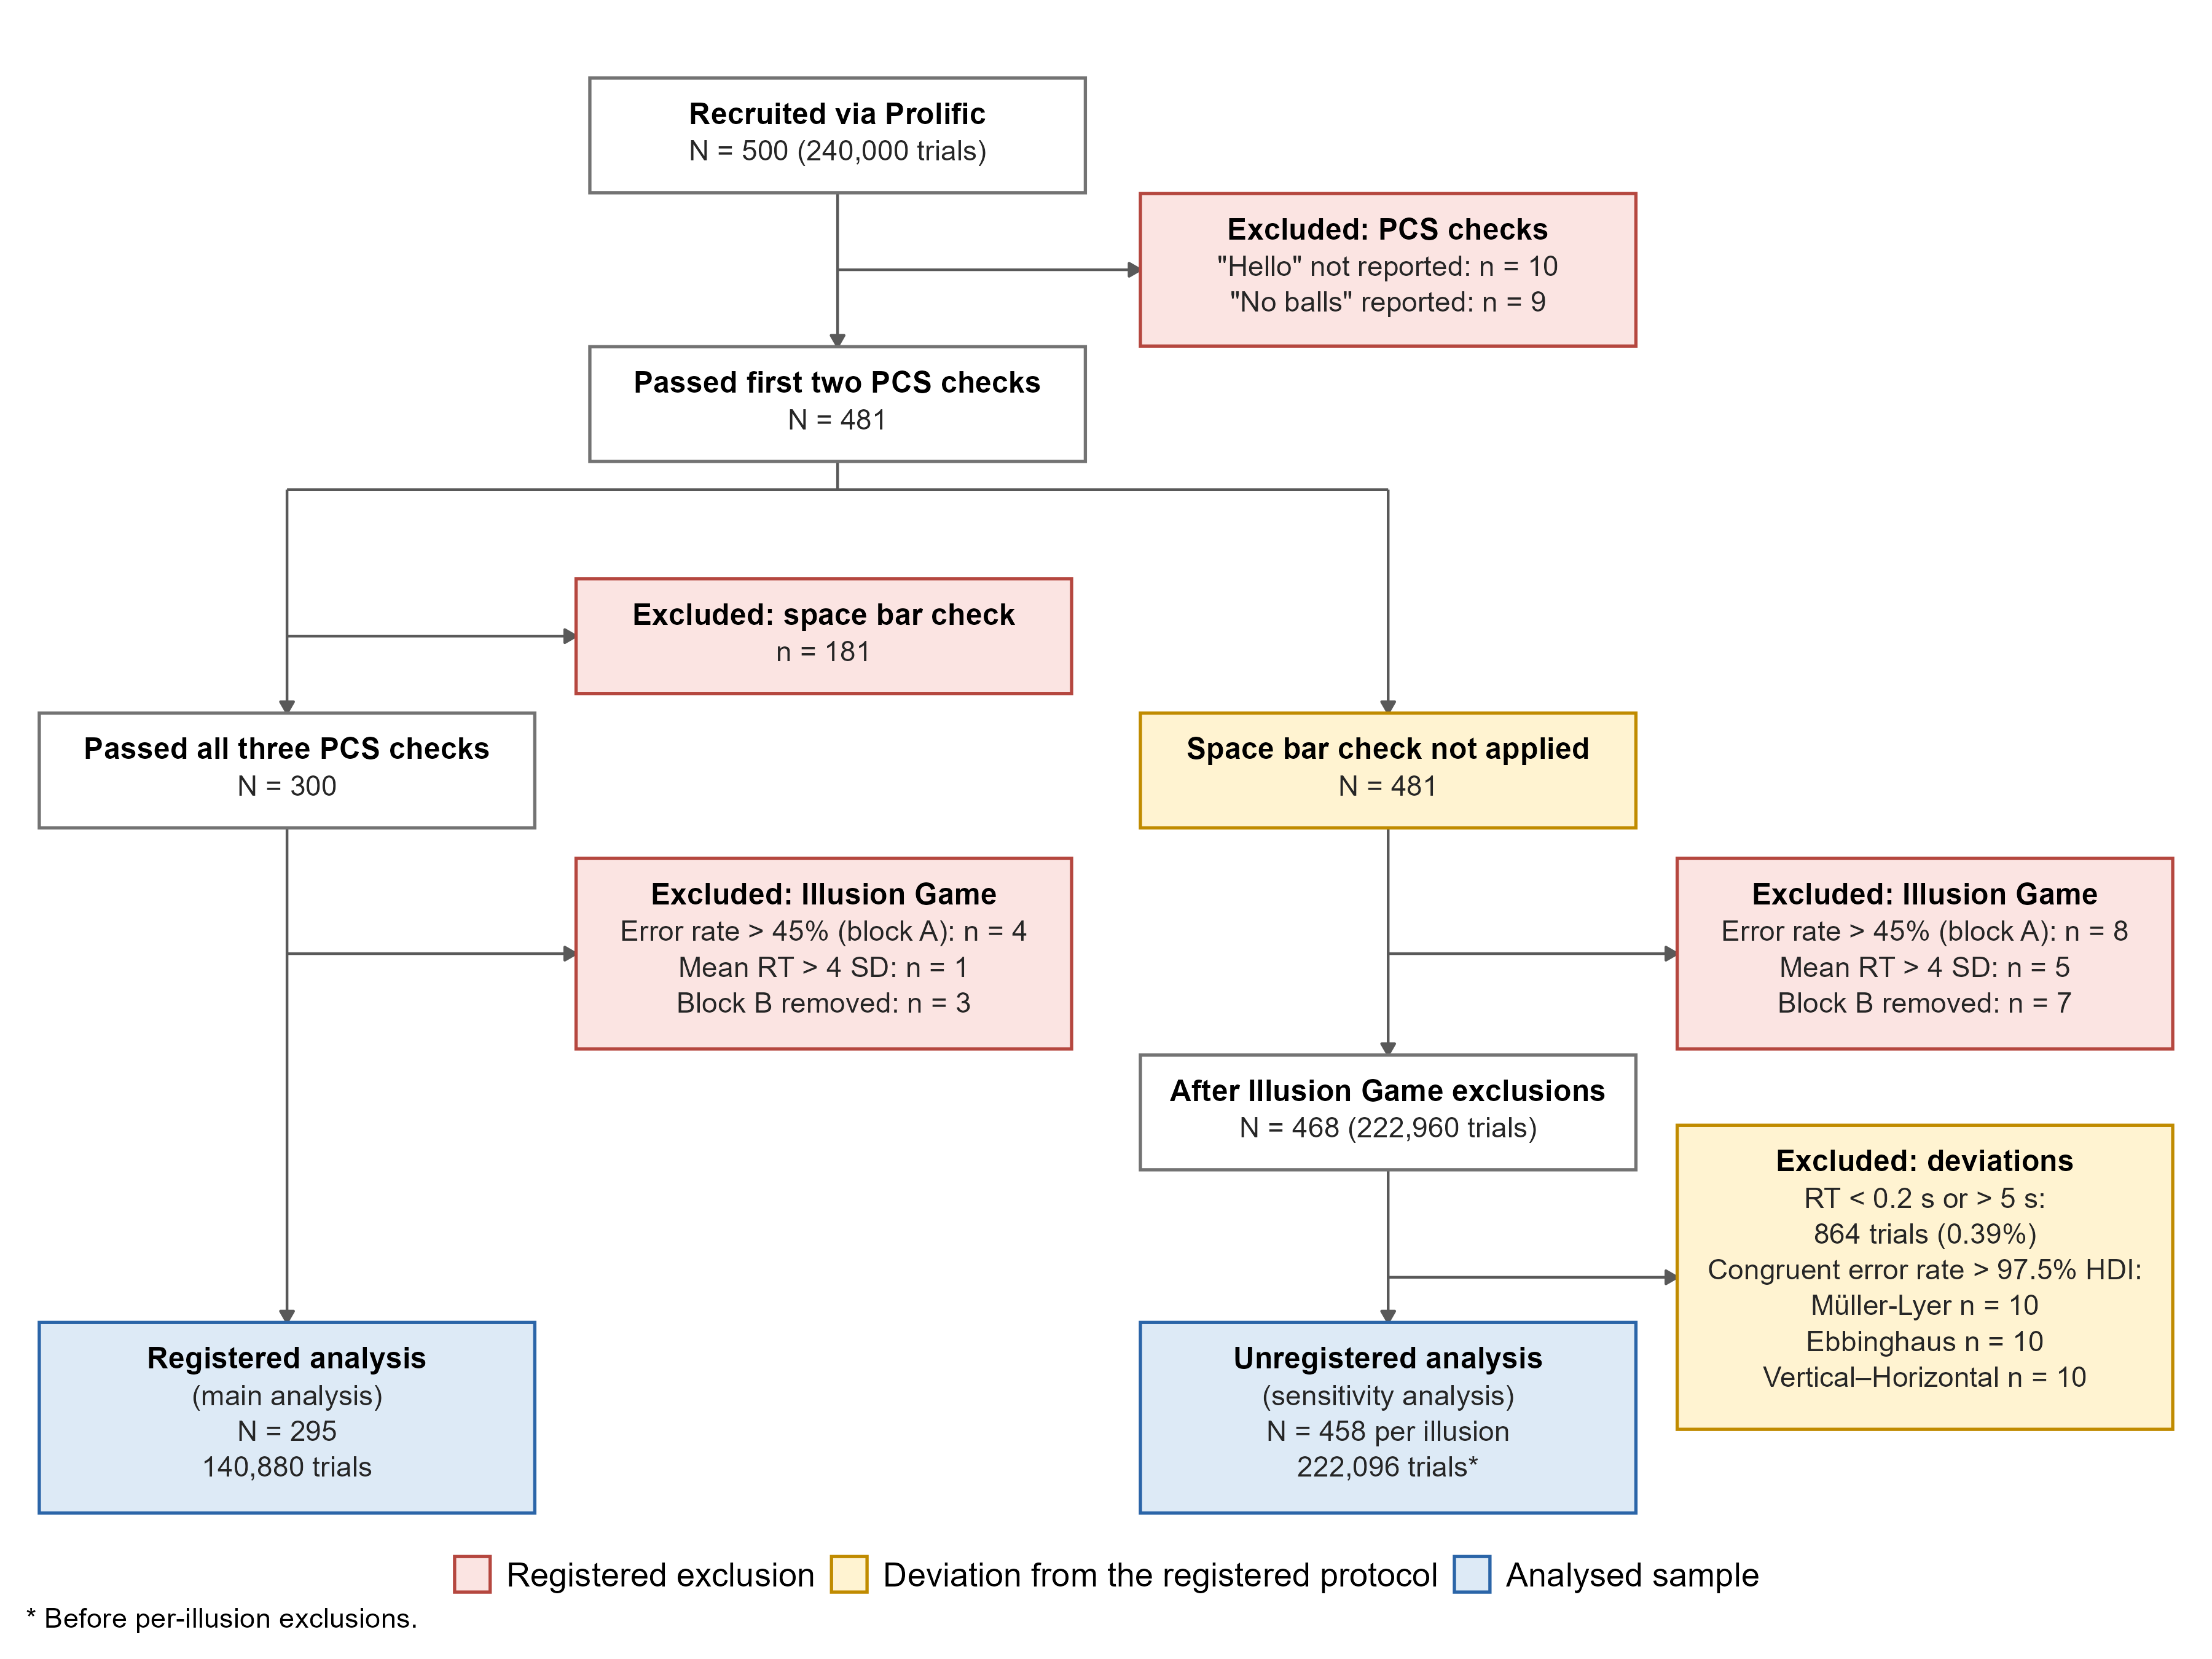
\includegraphics[width=1\linewidth,height=\textheight,keepaspectratio]{../../analysis/figures/fig_consort.png}

\textbf{Figure S2}

\textbf{\emph{Distribution of PCS and psychoticism scores in the
registered analysis (N = 295)}}

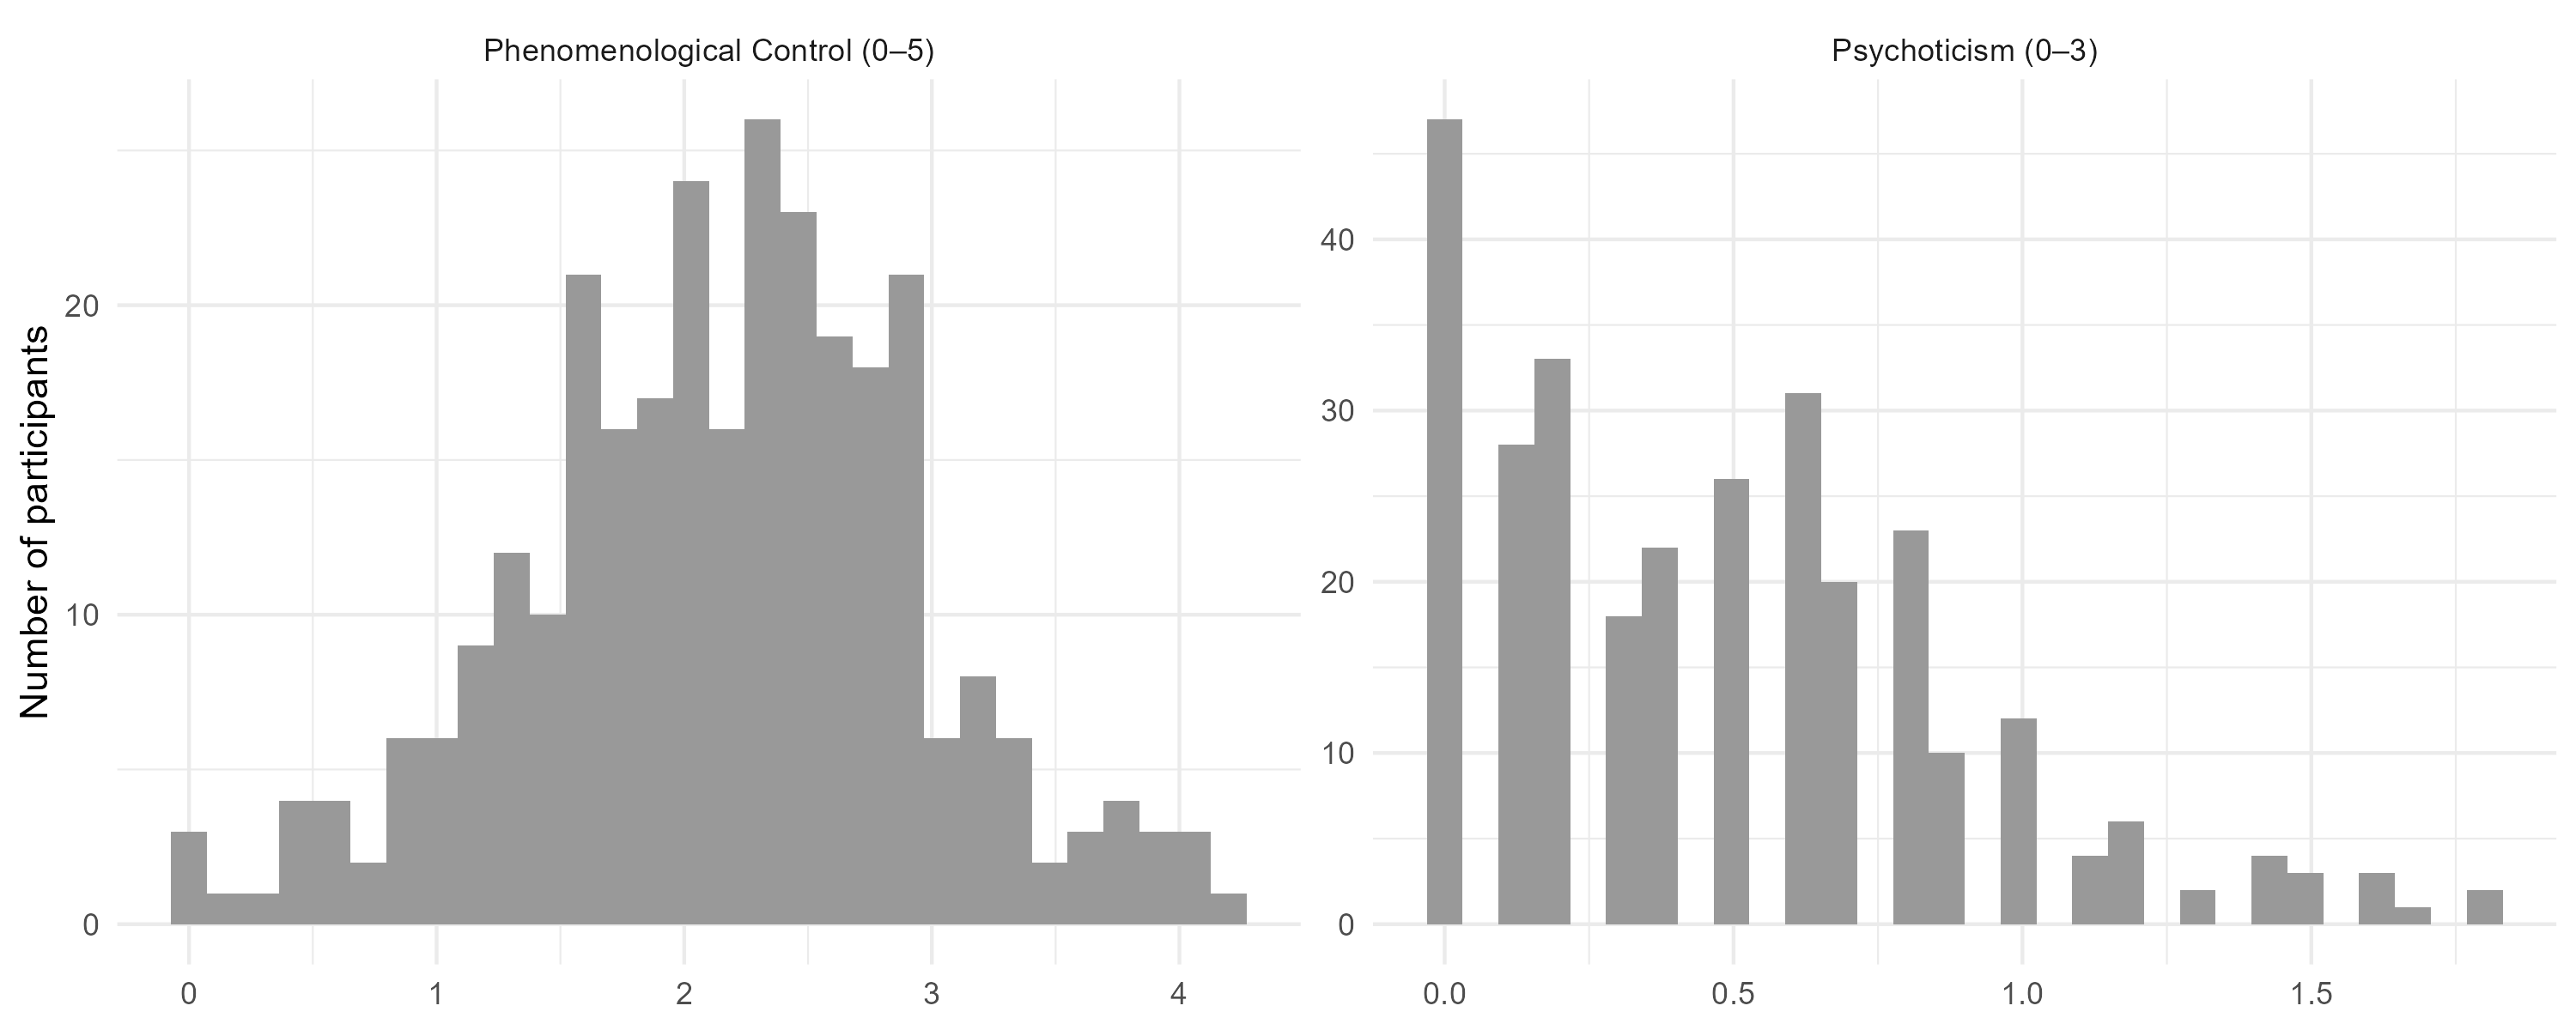
\includegraphics[width=1\linewidth,height=\textheight,keepaspectratio]{../../analysis/figures/fig_traits_distribution.png}






\end{document}
